%Preamble
\documentclass[12pt,oneside,letterpaper]{article}

% graphicx package, useful for including eps and pdf graphics
\usepackage{graphicx}
\DeclareGraphicsExtensions{.pdf,.png,.jpg}

% basic packages
\usepackage{color}
\usepackage{parskip}
\usepackage{float}

% make links a more pleasing color and don't box them
\definecolor{blue}{rgb}{0.85,0.70,0.99}
\usepackage[hidelinks]{hyperref}
\hypersetup{colorlinks=true,linkcolor=black,citecolor=black,urlcolor=blue}

% text layout
\usepackage{geometry}
\geometry{textwidth=15cm} % 15.25cm for single-space, 16.25cm for double-space
\geometry{textheight=22cm} % 22cm for single-space, 22.5cm for double-space

% helps to keep figures from being orphaned on a page by themselves
\renewcommand{\topfraction}{0.85}
\renewcommand{\textfraction}{0.1}

% bold the 'Figure #' in the caption and separate it with a period
% Captions will be left justified
\usepackage[labelfont=bf,labelsep=period,font=small]{caption}

% review layout with double-spacing
%\usepackage{setspace}
%\doublespacing
%\captionsetup{labelfont=bf,labelsep=period,font=doublespacing}

% cite package, to clean up citations in the main text
\usepackage{cite}

% Remove brackets from numbering in list of References
\renewcommand\refname{\large References}
\makeatletter
\renewcommand{\@biblabel}[1]{\quad#1.}
\makeatother

\usepackage{authblk}
\renewcommand\Authands{ \& }
\renewcommand\Authfont{\normalsize \bf}
\renewcommand\Affilfont{\small \normalfont}
\makeatletter
\renewcommand\AB@affilsepx{, \protect\Affilfont}
\makeatother

% notation
\usepackage{amsmath}
\usepackage{amssymb}

\renewcommand{\vec}[1]{\boldsymbol{#1}}
\newcommand{\Prob}{\mathbb{P}}
\newcommand{\Expect}{\mathbb{E}}
\newcommand{\Var}{\mathbb{V}}
\newcommand{\wt}{\text{wt}}
\newcommand{\var}{\text{var}}
\newcommand{\varE}{\text{escape}}
\newcommand{\varT}{\text{transmiss}}
\newcommand{\vac}{\text{vac}}

% Inline comments
\usepackage[normalem]{ulem}
\definecolor{purple}{rgb}{0.459,0.109,0.538}
\def\tbc#1{\textcolor{purple}{[#1]}}

\title{Transmission mechanisms determine relative fitness and frequency dynamics of viral variants}

\author[1,2,*]{Marlin D.\ Figgins}
\author[1,3]{Trevor Bedford}
\affil[1]{Vaccine and Infectious Disease Division, Fred Hutchinson Cancer Center, Seattle, WA, USA}
\affil[2]{Department of Applied Mathematics, University of Washington, Seattle, WA, USA}
\affil[3]{Howard Hughes Medical Institute, Seattle, WA, USA}
\affil[*]{Corresponding author: mfiggins@uw.edu}
\date{\today}
% https://maehler.se/blog/2013/11/01/authors-and-affiliations-in-latex

\begin{document}

\maketitle

% Longer abstract: \approx 250 words
% \begin{abstract}
%     Over the course of the COVID-19 pandemic, SARS-CoV-2 variants have repeated emerged, leading to large variant waves in populations of mixed immune backgrounds.
%     Classifying these variant viruses into genetically similar clades and lineages has allowed scientists to track the rise and fall of variants by modeling their frequencies over time.
%     These models of frequency dynamics allow us to estimate variant fitness advantages, however, these models typically cannot be interpreted at the level of transmission directly.
%     In this paper, we derive existing frequency dynamic models from exponentially growing populations and extend them to show that relative fitness of variants can be derived from compartment models of infectious diseases.
%     We use these models to illustrate how transmission mechanisms such as increased intrinsic transmissibility and immune escape can affect frequency dynamics, including trade-off between preferred mechanisms and complications identifying mechanism.
%
%     Motivated by this work, we develop a scalable approximate Gaussian process method for estimating relative fitness over time.
%     We, then, derive a selective pressure metric that estimates the contribution of frequency dynamics to population-level epidemic growth rates.
%     Using this metric, we are then able to develop a predictive model of epidemic growth rate from selective pressure.
%
%     We also propose a latent immunity space model for relative fitness which estimates pseudo-escape rates for variants and pseudo-immunity proportions for populations.
%     Applying this model to publicly available SARS-CoV-2 sequences globally, we estimate a pseudo-immunity landscape for SARS-CoV-2 variants.
%     These models offer novel insights into the mechanisms driving variant spread and have broad applicability to other rapidly evolution pathogens, enhancing our ability to understand viral populations from genetic sequences.
% \end{abstract}

% Short abstract: ~ 170 words
\begin{abstract}
    Since late 2020, emerging SARS-CoV-2 variants have repeatedly driven epidemics.
    Scientists have tracked these viral variants through phylogenetic approaches, classifying them into clades and lineages and modeling their frequencies over time to estimate their fitness advantages.
    However, these models typically cannot be interpreted at the level of transmission directly.
    We develop a general theory for existing frequency models and interpret fitness through compartment models of infectious disease, addressing trade-offs between immune escape and increased intrinsic transmissibility using frequency data.
    We introduce a scalable Gaussian process method for estimating relative fitness over time and develop a selective pressure metric which we use to predict epidemic growth rates from variant frequencies alone with a transformer-based prediction model.
    Additionally, we propose a latent immunity space model that estimates pseudo-escape rates for variants and pseudo-immunity proportions for populations, applying this model to publicly available SARS-CoV-2 sequences to map recent pseudo-immunity landscapes.
    These approaches offer novel insights into the mechanisms driving evolution in SARS-CoV-2 and can be applied to other rapidly evolving pathogens.
\end{abstract}


%TODO: References
% Huddleston et al, Antigenic waves, Cecile's paper, Usher, Obermyer, the one Jesse sent (?), Recent one ought of Sarah's lab, another talking about backboosting and original antigenic sin, immune dynamics cell paper
% Tegally, Tulio's lab, BA.2.12.1 paper
% Champredon paper on SE^nI^mR models so that we can extend to models with non-exponential generation times including latent periods .etc


% Introduction: ~718 words
\section*{Introduction}

%TODO: Flesh out, focusing on the emergence of looking at empirical variant advantage with frequency based model due to increased sequencing globally + tools like Nextclade.
%TODO: Include notes of desire to relate these frequency / selection estimates to transmission processes to understand risk posed by emerging variants

%TODO: Intro sentence about SARS-CoV-2

The COVID-19 pandemic has been marked by the successive emergence of SARS-CoV-2 variant viruses, driving repeated epidemics globally \cite{tegally2021detection, Volz2021}.
Though large waves have occurred repeatedly alongside the spread of novel variants, the underlying mechanism driving these waves appears to have changed over time.
Early mutations and viral variants such as Alpha, Beta, Gamma, Delta and their associated infection waves were largely driven by increases in intrinsic transmissibility which may be expected when there is lower population immunity.
%TODO: Citations: Bloom lab (Greaney Delta paper?)
The Omicron variant showed substantial immune escape and subsequent derived lineages within Omicron including XBB, EG.5.1, JN.1 appear to be driven by immune escape as evidenced through molecular studies of neutralization using human sera \cite{Cao2021, Cao2022, Bekliz2024, Jian2023}.
%TODO: Citations: Bloom lab?
Since 2022, there has been repeated replacement by subsequent Omicron-derived lineages.
This phenomenon of rapid viral population turnover is consistent with antigenic evolution and is observed in  other viruses such as seasonal influenza, although SARS-CoV-2 currently remains an outlier in terms of pace of its evolution \cite{Koel2013, Bedford2014, kistler2023atlas}.

Given the rapid emergence and spread of SARS-CoV-2 variants, it is important to assess the rate of turnover as this is an indicator of variant advantage and in addition to understanding how quickly a particular variant is spreading, it may signal the mechanism by which it spreads.
% With the increased temporal and geographical scale of sequencing that has occurred, we have gained more data than available for other circulating viruses giving a unique opportunity for insight into the evolution of SARS-CoV-2.
To estimate and understand variant turnover, frequency dynamic models of relative variant fitness have been developed.
These include simple models based on generalized linear models such as multinomial logistic regression, renewal-equation based methods, and various extensions based on hierarchical models or more careful treatments of variant emergence \cite{susswein2023leveraging, figgins2022sars, Piantham2022, Annavajhala2021, Lefrancq2023}.
These models estimate the relative fitness (or selective advantage) of circulating variant viruses from their frequency in sequencing data, typically represented by counts of variant sequences over time within a geographic region.
Relative fitness in these models is often assumed to be a constant quantity for simplicity and intrinsic to the variant of interest, however this may not be reasonable due to the nature of the transmission process.
Additionally, translating these relative fitness estimates to a population-level transmission advantage (in terms of variant infections per wildtype infection) typically requires assumptions on the generation time of the transmission though this can also be approached by jointly modeling the transmission process alongside frequencies \cite{Wallinga2006, figgins2022sars}.

It has been shown that population-level variant transmission advantages differ geographically and temporally which suggests that variant transmission advantages are not necessarily fixed or determined solely biologically and may be informed by within-region population differences \cite{figgins2022sars, vanDorp2022}.
In fact, they may be well explained by regional differences in immune structure as Dadonaite and co-authors show deep mutational scanning estimates are well correlated with estimated variant growth advantages \cite{Dadonaite2023}.
%TODO: Mention Voss paper and that if discrete # of antibodies based on exposure are genreated, we can think about immunity in temrs of past exposure histories
Existing models which allow for variation in variant transmission advantages generally do not have a mechanistic underpinning for why transmission advantages exist and vary geographically and temporally \cite{figgins2022sars, susswein2023leveraging}.
These non-mechanistic transmission advantages are useful for real-time situation analysis though more work is required to develop theory for how various mechanisms determine viral fitness.
In particular, distinguishing between mechanisms of immune escape and transmissibility may improve our ability to make informed short-term forecasts or include other forms of data to explain patterns of relative fitness.

% We introduce a theory of relative fitness and transmission advantages for exponentially growing populations.
% We then apply this to several ordinary differential equation models of epidemics to assess how different transmission mechanisms may contribute to variant turnover and describe relative fitness.
% Using these models, we then highlight the importance of historical population exposure, immune escape, and intrinsic transmissibility in determining variant turnover as well as short term forecasts of frequency growth.

Addressing this, we derive frequency dynamic models from exponentially growing populations and extend them using compartmental models of infectious diseases, providing a direct link between variant frequency dynamics and transmission mechanisms.
With the knowledge gained from this analysis, we develop several new models of variant frequency dynamics which we use to characterize trade-offs between intrinsic transmissibility and immune escape for pathogens showing that typically intrinsic transmissibility increases are preferred to immune escape due to low population exposure.
We then present a novel Gaussian process-based method for estimating time-varying fitness and introduce a selective pressure metric to quantify the impact of variant frequency dynamics on population-level epidemic growth rates.
Additionally, we employ a transformer-based prediction model that uses on selective pressure, derived from sequence counts alone, to forecast epidemic growth rates with high accuracy.
We also develop a latent immunity space model to estimate pseudo-escape rates and pseudo-immunity proportions, offering a comprehensive view of the immunity landscape.

\section*{Results}

\subsection*{Exponentially growing populations to frequency dynamics}%

We consider a viral population consisting of $V$ exponentially-growing variant viruses each with prevalence $I_{v}$.
Defining the time-varying growth rate for the prevalence of variant $v$ as $r_{v}(t)$, we can represent the prevalence using the following ordinary differential equation:

\begin{equation} \label{eq:inhomo_exp_growth}
    \frac{d I_{v}}{d t} = r_{v}(t) I_{v}(t), \quad v = 1,2, \ldots, V.
\end{equation}

The above differential equation has a known solution in terms of the integral of the time-varying growth rate and initial prevalence as follows:

\begin{align*}
I_{v}(t) = I_{v}(0) \exp\left( \int_{0}^{t} r_{v}(s) ds\right),
\end{align*}
where $I_{v}(0)$ is the initial prevalence of variant $v$.

Now turning to the frequency dynamics of the population, we write the frequency of variant $v$ in the population as  $f_{v}(t) = I_{v}(t) / \sum_{u=1}^{V} I_{u}(t)$.
This allows us to derive an ODE for variant frequency in terms of the variant growth rates using the quotient rule for differentiation:
\begin{align*}
    \frac{d f_{v}}{d t} &= f_{v} \left( \sum_{u=1}^{V} [r_{v}(t) - r_{u}(t)] f_{u} \right)\\
                        &= f_{v} \left( r_{v}(t) - \sum_{u=1}^{V} r_{u}(t) f_{u} \right).
\end{align*}

This system of differential equations resembles a logistic growth equation and can be shown to have the following solution in terms of the initial frequencies $f_{v}(0)$ and the variant growth rates:
\begin{align}
    f_{v}(t) &= \frac{ f_{v}(0) \exp( \int_{0}^{t} r_{v}(s) ds)}{\sum_{u=1}^{V}  f_{u}(0) \exp( \int_{0}^{t} r_{u}(s) ds)}.
\end{align}

The above representation of the variant frequency will serve as a centerpiece for many of the arguments to follow.
We see that by tracking the rate at which variant viruses are spreading, we can construct the corresponding frequency dynamics without knowing the absolute prevalence of any variant.

\paragraph{Relative frequency and relative fitness}%

Using the above equation for the variant frequencies, we can write the relative frequency of variant $v$ over $u$ as $x_{v,u}(t) = f_{v}(t) / f_{u}(t)$ to see:
\begin{align*}
    x_{v, u}(t) = \frac{f_{v}(t)}{f_{u}(t)} &= \frac{f_{v}(0)}{f_{u}(0)} \exp \left( \int_{0}^{t} [r_{v}(s) - r_{u}(s)] ds \right)\\
                                            &=x_{v,u}(0)\exp \left( \int_{0}^{t} \lambda_{v,u}(s) ds \right).
\end{align*}

Notice this relative frequency change depends on the initial relative frequencies and the \emph{relative fitness} $\lambda_{v,u}(t) = r_{v}(t) - r_{u}(t)$ of $v$ over $u$.
This relative fitness has the same units as the exponential growth rate (e.g. per day). 
Using the definition of relative fitness, we can notice that
\begin{align}
\lambda_{v, u}(t) = r_{v}(t) - r_{u}(t) = \frac{d }{d t} \left[\log \left( x_{v,u}(t) \right) \right] = - \lambda_{u,v}(t)
\end{align}

We can see that there is a symmetry in the relative fitnesses and that the associated frequency dynamics depend on the differences between relative fitnesses.
This suggests that absolute fitness (in terms of the growth of infections) may not be inferable from frequencies alone.
This definition of relative fitness becomes essential in describing various existing modeling approaches for frequency dynamic data and motivates possible extensions since we can represent these models as having the form:
\begin{align}
    f_{v}(t) &= \frac{ f_{v}(0) \exp( \int_{0}^{t} \lambda_{v, \text{pivot}}(s) ds)}{\sum_{u=1}^{V}  f_{u}(0) \exp( \int_{0}^{t} \lambda_{u, \text{pivot}}(s) ds)},
\end{align}
where the growth rate of $v$ is expressed as relative to an arbitrary pivot variant.

\paragraph{Cumulative relative-fitness and frequency change}

Above we saw that within our framework frequency change over time intervals depends only on the cumulative relative fitness over time intervals $\Lambda_{v,u}(0, t) = \int_{0}^{t} \lambda_{v, u}(s)ds$.
We can then characterize approaches for modeling frequency change in terms of how they represent, estimate, and forecast these relative fitnesses.
This framework includes various existing methods for analyzing frequency data such as the seasonal influenza forecasting models of L{\"a}ssig and {\L}uksza \cite{luksza2014predictive} and Huddleston et al \cite{Huddleston2020}, multinomial logistic regression for frequency estimation \cite{Annavajhala2021} and the SARS-CoV-2 mutational fitness model of Obermeyer et al \cite{Obermeyer2022}.
%Question: How would I nest Piantham in this framework? Can I?

Though this framework can be used to describe existing statistical methods for frequency modeling, it is also applicable to traditional compartmental models of epidemics.
In fact, applying these ideas to compartmental models enables to see how mechanistic assumptions on the transmission process determine relative fitness of variant viruses.

\subsection*{Transmission mechanisms determine relative fitness of variants}

Multi-strain models of epidemics have been developed to understand the competition between different viral strains that exhibit different levels of cross-immunity \cite{Gog2002, Wen2022}.
These models have typically been used to explain strain evolution in antigenically variable pathogens like seasonal influenza \cite{Bedford2014} and seasonal coronaviruses OC43 and 229E \cite{Kistler2021, Eguia2021}.

In order to better understand frequency dynamics of pathogens with multiple co-circulating variants, we can apply the above framework to compartmental models of epidemics which can be written in the form of Equation~\ref{eq:inhomo_exp_growth}.
These models will provide us with an intuition of how strain-level selection depends on the assumed transmission mechanism of the underlying epidemic model.

\paragraph{Two-strain SIR}%

For simplicity, we will begin by analyzing a two-strain SIR model in which the a variant virus $v$ can differ from wildtype virus wt by increased intrinsic transmissibility (via $\eta_{T}$) and immune escape against wild-type immunity (via $\eta_{E}$).
This system of 5 ordinary differential equations follows

%TODO: Add 3.x
\begin{align*}
    \frac{d S}{d t} &= - \beta S I_{\wt} - \beta \eta_{T} S I_{v}\\
    \frac{d I_{\wt}}{dt} &= \beta S I_{\wt} - \gamma I_{\wt}\\
    \frac{d I_{v}}{dt} &= \beta \eta_{T} S I_{v} + \beta \eta_{T} \eta_{E} \phi_{\wt} I_{v} - \gamma I_{v}\\
    \frac{d \phi_{\wt}}{dt} &= \gamma I_{\wt} - \beta \eta_{T} \eta_{E} \phi_{\wt} I_{v}\\
    \frac{d \phi_{v}}{dt} &= \gamma I_{v}.
\end{align*}
where $I_{\wt}$ denotes wild-type prevalence, $I_{v}$ denotes variant prevalence and $\phi_{\wt}$ denotes immunity derived from wild-type infection.
In this model, the variant virus can infect both susceptible individuals $S$ and individuals with immunity to wild-type virus $\phi_{\wt}$.
Increased intrinsic transmissibility increases the baseline transmission rate from $\beta$ in wild-type to $\beta \eta_{T}$ in the variant virus and immune escape increases the transmission rate against those with wildtype immunity, so that the at-risk population is $\eta_{E} \phi_{\wt}$.

Writing that $r_{\wt}(t) = \beta S - \gamma$ and $r_{v}(t) = \eta_{T} \beta  S + \beta \eta_{T} \eta_{E} \phi_{\wt} - \gamma$, we can then write the relative fitnesses as:
\begin{equation} \label{eq:two_strain_relative_fitness}
\lambda_{v,\wt}(t) = (\eta_{T} - 1)\beta S(t) + \eta_{T} \eta_{E} \beta \phi_{\wt}(t).
\end{equation}

From this representation of relative fitness, we can see that given fixed increases to overall transmission ($\eta_{T} > 1$) or immune escape ($\eta_{E} > 0$), the observed fitness boost at the level of variant relative fitness still depends on the proportion of the population at risk for infection.

\paragraph{$n$-strain SIR}%

This model can also be extended to an $n$-strain SIR model where each variant strain $v_i$ with $2\leq i \leq n$ is described by its own advantage parameters $\theta_{i} = (\eta_{T}^{(i)},\eta_{E}^{(i)})$  relative to the wildtype ($\theta_{\text{wt}} = \theta_{1} = (0, 0)$).

\begin{align*}
    \frac{d S}{d t} &= - \beta S I_{\wt} - \beta \eta_{T} S I_{v_{i}}\\
    \frac{d I_{\wt}}{dt} &= \beta S I_{\wt} - \gamma I_{\wt}\\
    \frac{d I_{v_{i}}}{dt} &= \beta \eta_{T, i} S I_{v_{i}} + \beta \eta_{T, i} \eta_{E, i} \phi_{\wt} I_{v_{i}} - \gamma I_{v_{i}}\\
    \frac{d \phi_{\wt}}{dt} &= \gamma I_{\wt} - \beta \eta_{T, i} \eta_{E, i} \phi_{\wt} I_{v_{i}}\\
    \frac{d \phi_{v_{i}}}{dt} &= \gamma I_{v_{i}}, \quad i \in \{2, \ldots, n\}.
\end{align*}

In this formulation, the variant viruses compete only for susceptible population and those with previous wild-type infection.
This formulation can be generalized to allow for competition between all variants for any exposure history and will be discussed in the following sections.
In Figure \ref{fig:vis_mechanisms}, we implement and simulate a 3-strain model with wildtype as above, an escape variant E with $\theta_{2} = (0, \eta_{E})$, and a transmissibility increase variant T with $\theta_{3} = (\eta_{T}, 0)$.
% \tbc{I'm confused on the units of relative fitness. If $r_{v}(t)$ has units of `per day', then relative fitness will also be `per day'? I ran into this in trying to get a sense of the scale of fitness differences in Figure 1.}
% I've added a discussion about units when I define relative fitness. I can also do this when we define the exponential growth rate as well

\begin{figure}[h]
    \centering
    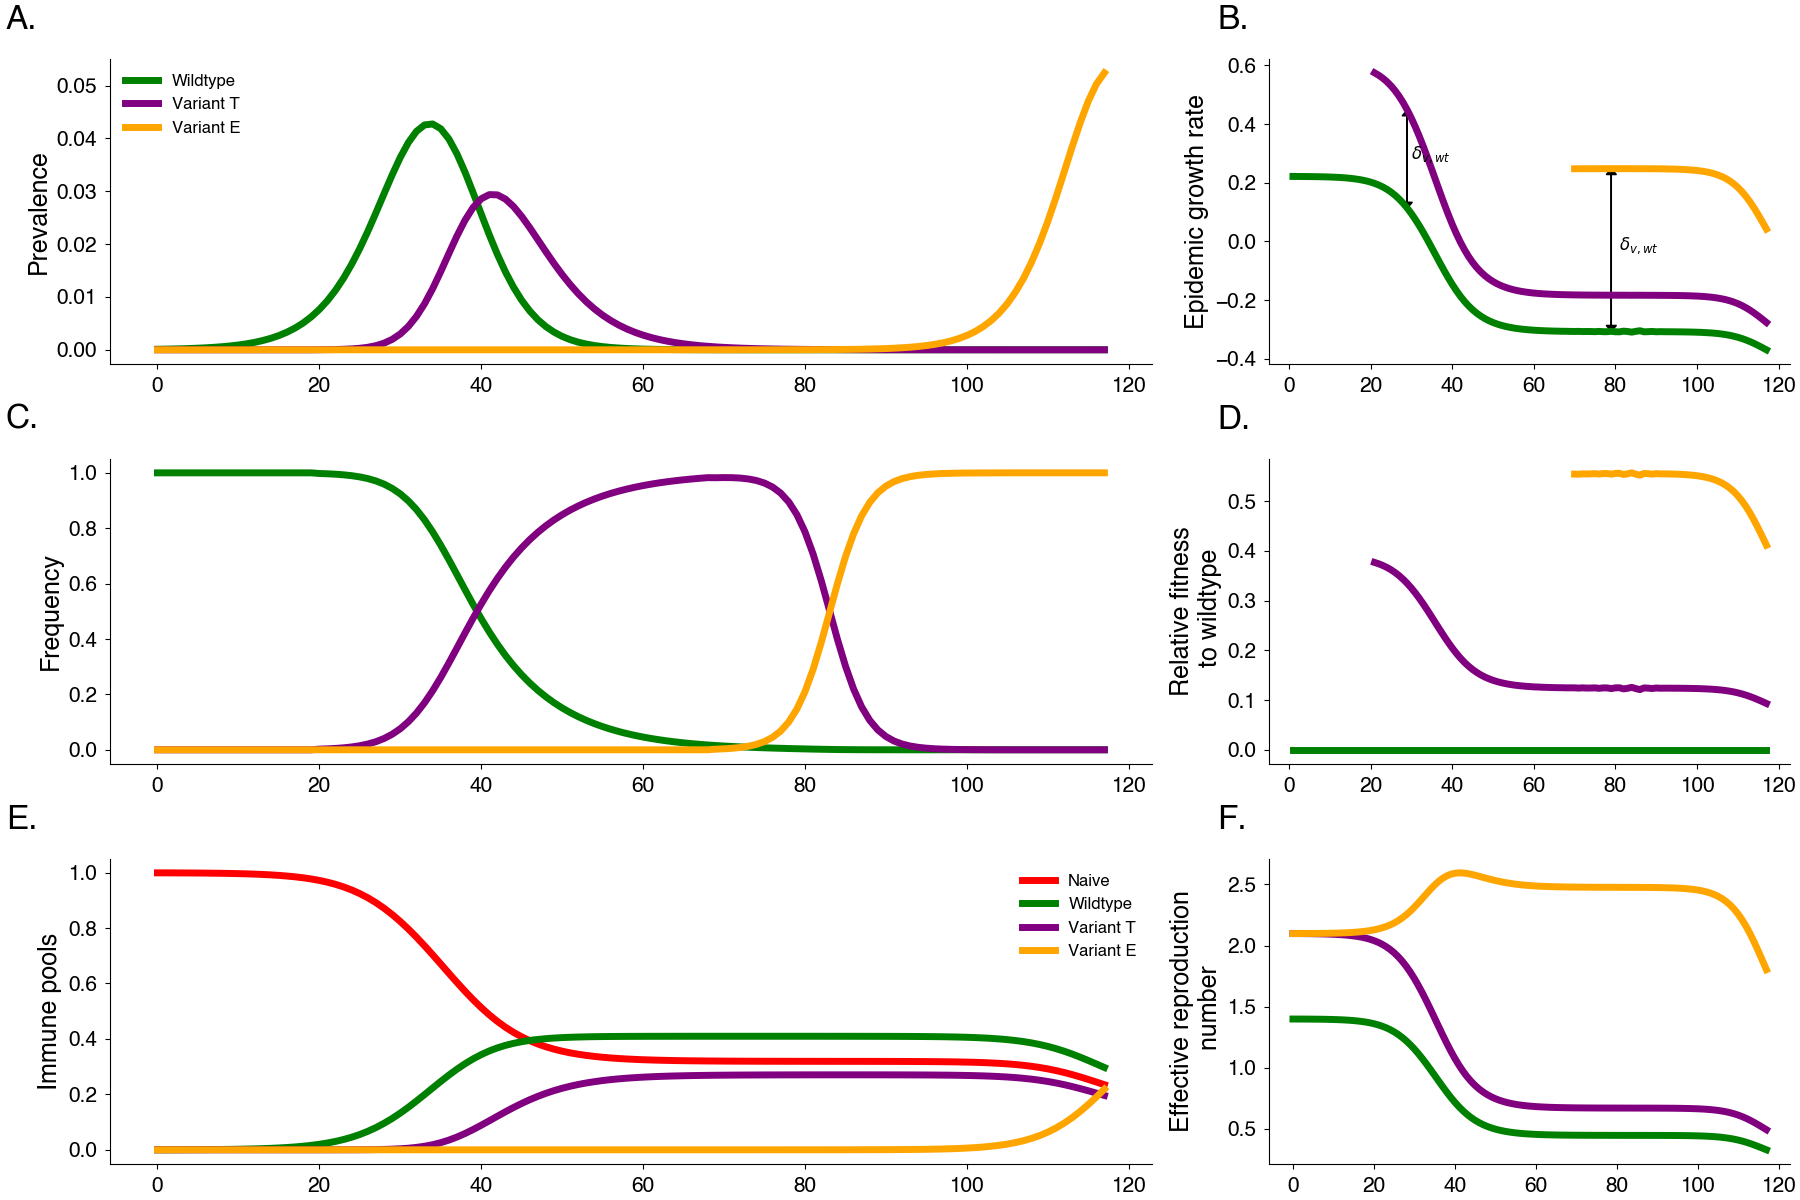
\includegraphics[width=1.0\linewidth]{./figures/vis_mechanisms.png}
    \caption{\textbf{Method overview.}
    Mechanistic transmission models constrain variant frequency dynamics by specifying a functional form for relative fitnesses.
    Simulations of a three-variant model including a wildtype, one intrinsic transmission increased variant, and one immune escape variant show the relationship between population-level transmission and selection for variants.
    We begin the simulation with initial wildtype frequency $10^{-4}$, $R_{0,\wt} = 1.4$, and $\gamma^{-1} = 1.8$.
    We introduce the transmissibility variant at $t=20$ with $\eta_T = 1.5$ and initial frequency $10^{-5}$, and introduce the escape variant at $t=70$ with $\eta_E = 1.05$ and initial frequency $10^{-6}$.
    A. Prevalence by variant.
    B. Exponential growth rate by variant.
    C. Variant frequency.
    D. Relative fitness relative to wildtype.
    E. Underlying immune pools.
    F. Effective reproduction number by variant.
    % \tbc{It's a little confusing having the left-hand panels be so much wider than the right-hand panels when they share exactly the same x-axis. I'd suggest to make left and right panels equal widths.}
    % \tbc{I'm confused on why variant E has growth rate $r$ and relative fitness $\lambda$ only measured starting at time = $\sim$70, while reproductive number $R$ is measured from time = 0. Ie if you can measure $R$, can't you also measure $r$?}
    % \tbc{Include in legend the initial frequencies / prevalences of the three variants as well as the values of $\eta_{E}$ and $\eta_{T}$.}
    % \tbc{It would be nice to have y-axis for proportions in panels C and E be labeled 0\%, 20\%, etc\ldots, instead of 0.0, 0.20, etc\ldots.}
    % \tbc{It would be nice to connect your notation here, where panel B would read `Epidemic growth rate $r$' and panel D would read `Relative fitness to wildtype $\lambda$'}
}%
    \label{fig:vis_mechanisms}
\end{figure}

\paragraph{Models of immune escape against heterogeneous backgrounds}%

We'll now consider a model where all hosts are assumed to fall into one of $B$ immune backgrounds $\phi_{b}$ for $b =1, \ldots, B$.
We assume that infection by each variant $v$ then leaves recovered hosts in the corresponding immune background of the most recent infection $b_{v}$.
Variant transmission then occurs via immune escape against a background leading to a matrix of escape rates $\vec{\eta} = \eta_{v,b}$ for variants $v$ and background $b$.

We can then write the system of ordinary differential equations as
\begin{align*}
    \frac{d I_{v}}{dt} &= \beta \sum_{1\leq b \leq B} \eta_{v, b} \phi_{b} I_{v} - \gamma I_{v}, \quad v = 1, \ldots, V\\
    \frac{d \phi_{b}}{dt} &= - \beta \sum_{1\leq v \leq V} \eta_{v,b}\phi_{b} I_{v} +  \sum_{v:\ b_{v} = b} \gamma I_{v}.
\end{align*}

With this model, susceptible and recovered compartments in the standard SIR model can be thought of as immune backgrounds.
This allows us to represent the standard SIR model as $S = \phi_{S}$, $I = I_{\wt}$, $R = \phi_{\wt}$ and $\eta_{\wt, S} = 1, \eta_{\wt, \wt} = 0$ and $b_{\wt} = \wt$.
We can also think of the two-strain SIR with $\eta_{T} = 1$ as a special case of this model where we set $S = \phi_{S}, \eta_{\wt, S} = 1, \eta_{\wt, \wt} = 0, \eta_{v, S} = 1, \eta_{v, \wt} = \eta_{E}$ and keep all other parameters the same.

With this formulation of immune escape, we can then write the relative fitnesses in terms of the escape rates $\eta_{v,b}$ and the immune background proportions $\phi_{b}$ as

\begin{equation} \label{eq:escape_relative_fitness}
    \lambda_{v, u}(t) = \beta \sum_{1\leq b \leq B}(\eta_{v,b} - \eta_{u,b}) \phi_{b}(t).
\end{equation}

Under this model of immune escape, we can see relative fitness among variants can be decomposed into differences in immune escape among immune backgrounds within a population.
Due to the dependence here on the proportion of each immune background in determining fitness, this suggests that the overall distribution of susceptibility to strains is potentially an important consideration when translating individual-level measures of immune escape to population-level estimates of variant fitness.
Understanding the size and complexity of this immune space may therefore be useful for parameterization and forecasting of variant frequencies.
However, the extent to which modeling this complexity affects estimates of relative fitness also depends on how quickly the distribution of immune backgrounds change i.e. $\frac{d\phi_{b}}{dt}$.

Though the derivation above uses a simplified model of using most recent infection to sort individuals into an immune group, we show that a more complicated model that accounts for the entire exposure history of the host also gives a similar decomposition to relative fitness in Supplemental Appendix \ref{ssec:full_immune_history}.

\section*{Applications}

Using the theory developed for exponentially-growing variant populations, we now re-visit existing methods for modeling viral frequency dynamics.

\paragraph{Multinomial Logistic Regression}%

We begin with multinomial logistic regression (MLR) with fixed relative fitness.
This model can be written as

\begin{align*}
    f_{v}(t) = \frac{f_{v}(0) \exp(\lambda_{v} t)}{\sum_{u} f_{u}(0) \exp(\lambda_{u} t)},
\end{align*}

where $f_{v}(t)$ is the frequency of variant $v$ at time $t$ and $\lambda_{v}$ is the relative fitness of variant $v$.
This provides estimates of the relative fitness compared to some reference strain $u^{*}$ for which $\lambda_{u^*} = 0$.
In this model, initial frequencies $f_{v}(0)$ and relative fitness $\lambda_{v}$ are estimated from frequency dynamics.
Converting this estimate to an estimate of transmission advantage (relative effective reproduction number) requires assuming a delta distribution of the generation time \cite{Wallinga2006}.

By comparison to equation \ref{eq:two_strain_relative_fitness}, we can see this model of fixed relative fitness results from assuming that the at-risk populations are constant over-time.
This assumption is useful since it requires no outside knowledge of the at-risk population and relative infection rates, though this may be less useful for longer forecasts or when there is large turnover in at-risk populations due to infection.

\paragraph{Fitness models of seasonal influenza}%

Motivated by the observed antigenic evolution of seasonal influenza, L{\"a}ssig and {\L}uksza \cite{luksza2014predictive} and Huddleston et al \cite{Huddleston2020} approximate the cumulative relative fitness between influenza seasons on the level of individual strains as

\begin{align*}
    \Lambda_{v,u}(t + \Delta t,t) = (\beta_{1} x_{v,1} + \cdots + \beta_{p} x_{v, p})\Delta t = (\vec{\beta} \cdot \vec{x}_{v}) \Delta t,
\end{align*}

where the relative fitness is determined by strain-specific predictors $\vec{x}_{v}$ and the regression parameter $\vec{\beta}_{v}$ are estimated. 

This formulation fits neatly into the framework we've developed as the cumulative fitness here can be written as the integral of a relative fitness $\lambda_{v, u} =  \vec{\beta} \cdot \vec{x}_{v}$ over the time period of interest:

\begin{align*}
    \Lambda_{v,u}(t + \Delta t,t)  &= \int_{t}^{t+\Delta t} \lambda_{v,u}(s)ds\ = \int_{t}^{t + \Delta t} (\vec{\beta} \cdot \vec{x}_{v}) ds.
\end{align*}

Therefore, these models can be thought as regression-based predictors of relative fitness where frequency and external covariates contribute to estimated relative fitness.

% \tbc{There needs to be more of a point here. Spell out how $\lambda$ in this model relates to your $\lambda$. I think of this like MLR, but where relative fitnesses are fixed from coefficients rather than learned from frequencies.}
% The authors choose predictors which describe the antigenic properties of strains

\paragraph{Estimating relative fitness using Gaussian Processes}%

We develop a method for using Gaussian processes to model variant relative fitness.
Gaussian processes are probability distributions over functions, where the structure and smoothness of these functions are defined by a kernel that encodes correlations in time.
These models are flexible and allow us to encode smoothness constraints, periodicity, and other structures \cite{Görtler2019a}.
Here, the relative fitnesses are modeled using an approximate Gaussian process with a Matern 5/2 kernel and shared hyperparameters across variants.
For efficiency, we implement a Hilbert Space Gaussian Process (HSGP) approximation instead of fitting $V$ independent Gaussian processes since the HSGP allow us to share basis functions \cite{riutortmayol2022practical}.
This model is used in Figure \ref{fig:gp_example} to estimate the relative fitnesses of different variants through time $\lambda_v(t)$ based on simulated variant sequence counts from frequencies shown in Figure \ref{fig:vis_mechanisms}.

\begin{figure}[h]
    \centering
    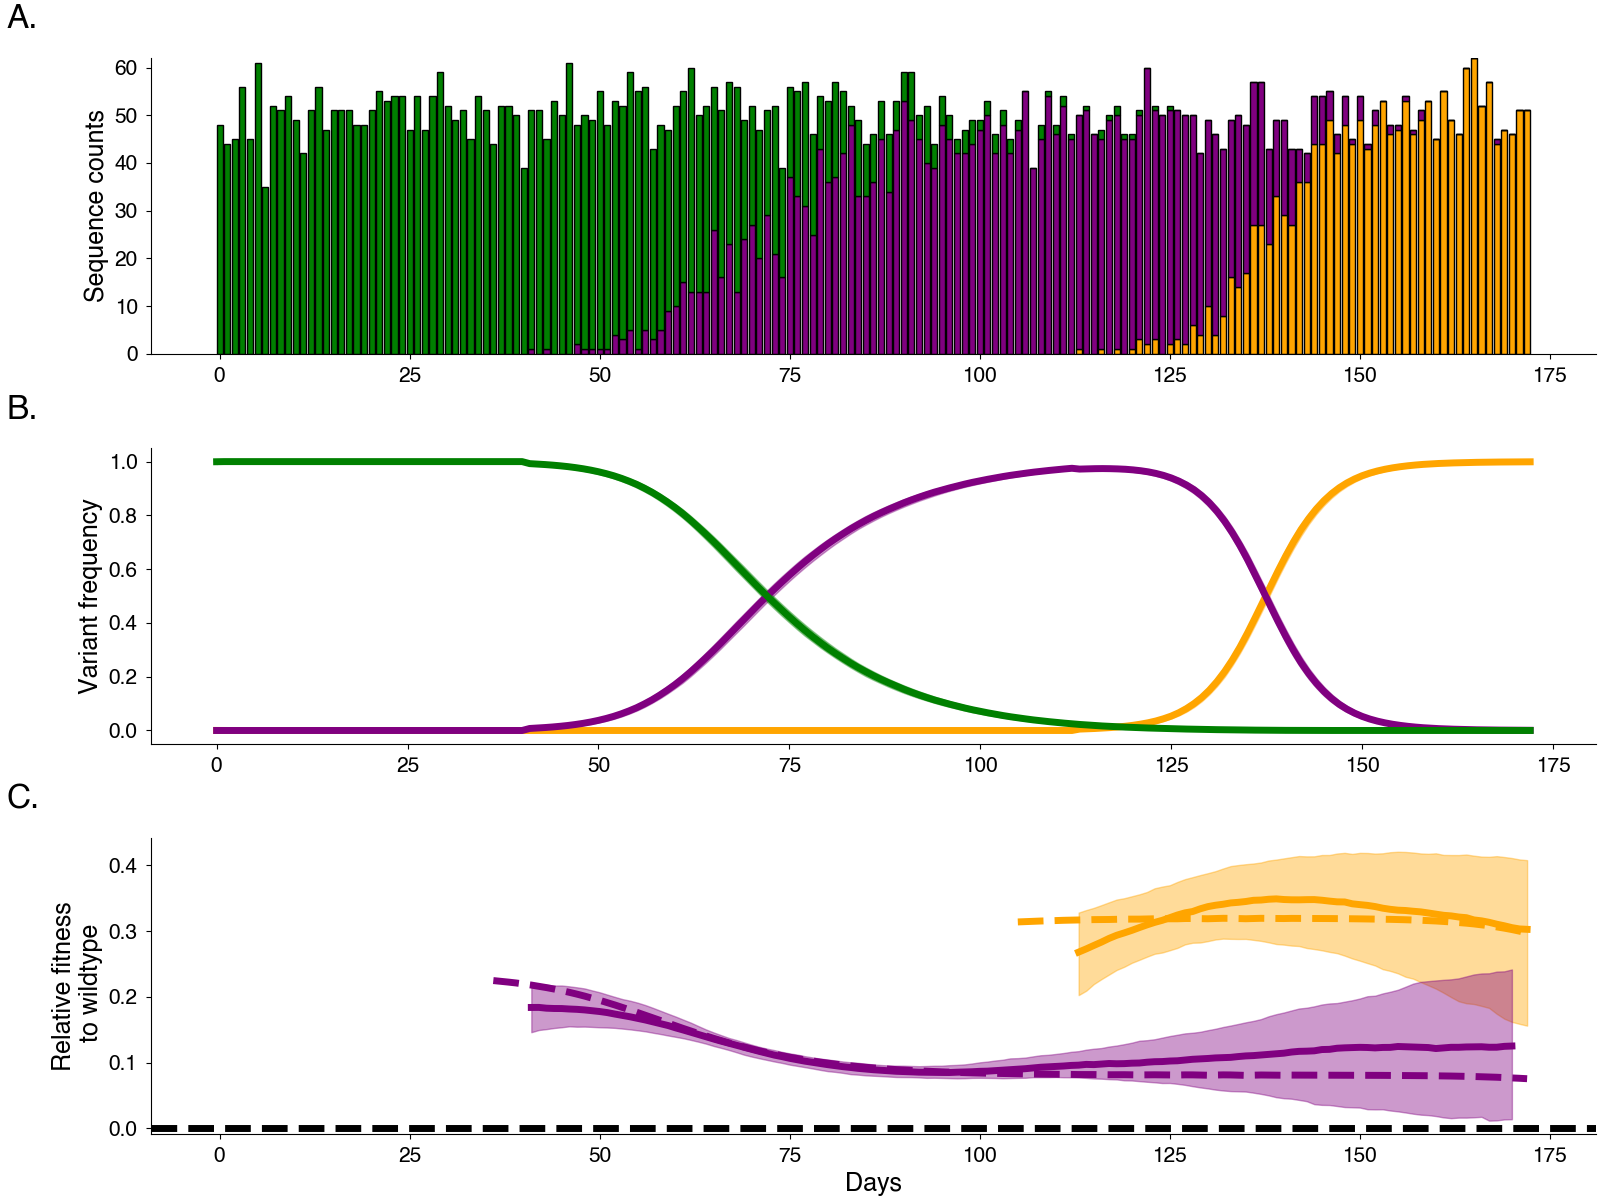
\includegraphics[width=0.8\linewidth]{./figures/gp_example.png}
    \caption{\textbf{Estimating relative fitness with Gaussian Processes.}
    Gaussian processes allow us a non-parametric estimate of the relative fitness for variants through time.
    This figure uses Gaussian processes to model the 3 variant example shown in Figure \ref{fig:vis_mechanisms}.
    A. Synthetic sequence counts generated using a multinomial distribution with frequencies from Figure \ref{fig:vis_mechanisms}C.
    B. Frequencies and posterior frequencies according to Gaussian process model. Intervals show the 80\% credible interval.
    C. Relative fitnesses. Dashed line shows true relative fitnesses from underlying mechanistic model.
}
    \label{fig:gp_example}
\end{figure}


\paragraph{Transmisibility-Escape Tradeoff}%

Extending this analysis to two variant viruses $v= \wt, \varE, \varT$ such that $\eta_{T}^{\varE} = 1$ and $\eta_{E}^{\varT} = 0$, we can write relative fitnesses an escape only variant or transmissibility increased variant as
\begin{align*}
    \lambda_{\varE, \wt} &= \eta_{E} \beta \phi_{\wt}(t)\\
    \lambda_{\varT, \wt} &= (\eta_{T} - 1) \beta S(t).
\end{align*}

In the simplest case where individuals are either susceptible or have wildtype immunity ($S(t) + \phi_{w}(t) = 1$), we can compute the critical immune fraction $\phi^{*}$ at which $\lambda_{\varE, w}(\phi^{*}) = \lambda_{\varT, w}(\phi^{*})$ as
\begin{equation} \label{eq:critical_immunity}
    \phi^{*} = \frac{\eta_{T} - 1}{\eta_{E} + \eta_{T} - 1}.
\end{equation}

For past exposure level greater than $\phi^{*}$, escape variant have a higher relative fitness.
This trade off shows that increasing escape rate entails that a lower proportion of past exposure is needed for escape variants to be preferred (Figure \ref{fig:transmission_tradeoff}).
Additionally, this shows that when intrinsic transmissibility increases are limited escape is more likely to be a dominant mechanism for variant turnover.

We visualize this trade-off in Figure \ref{fig:transmission_tradeoff}.

\begin{figure}[h]
    \centering
    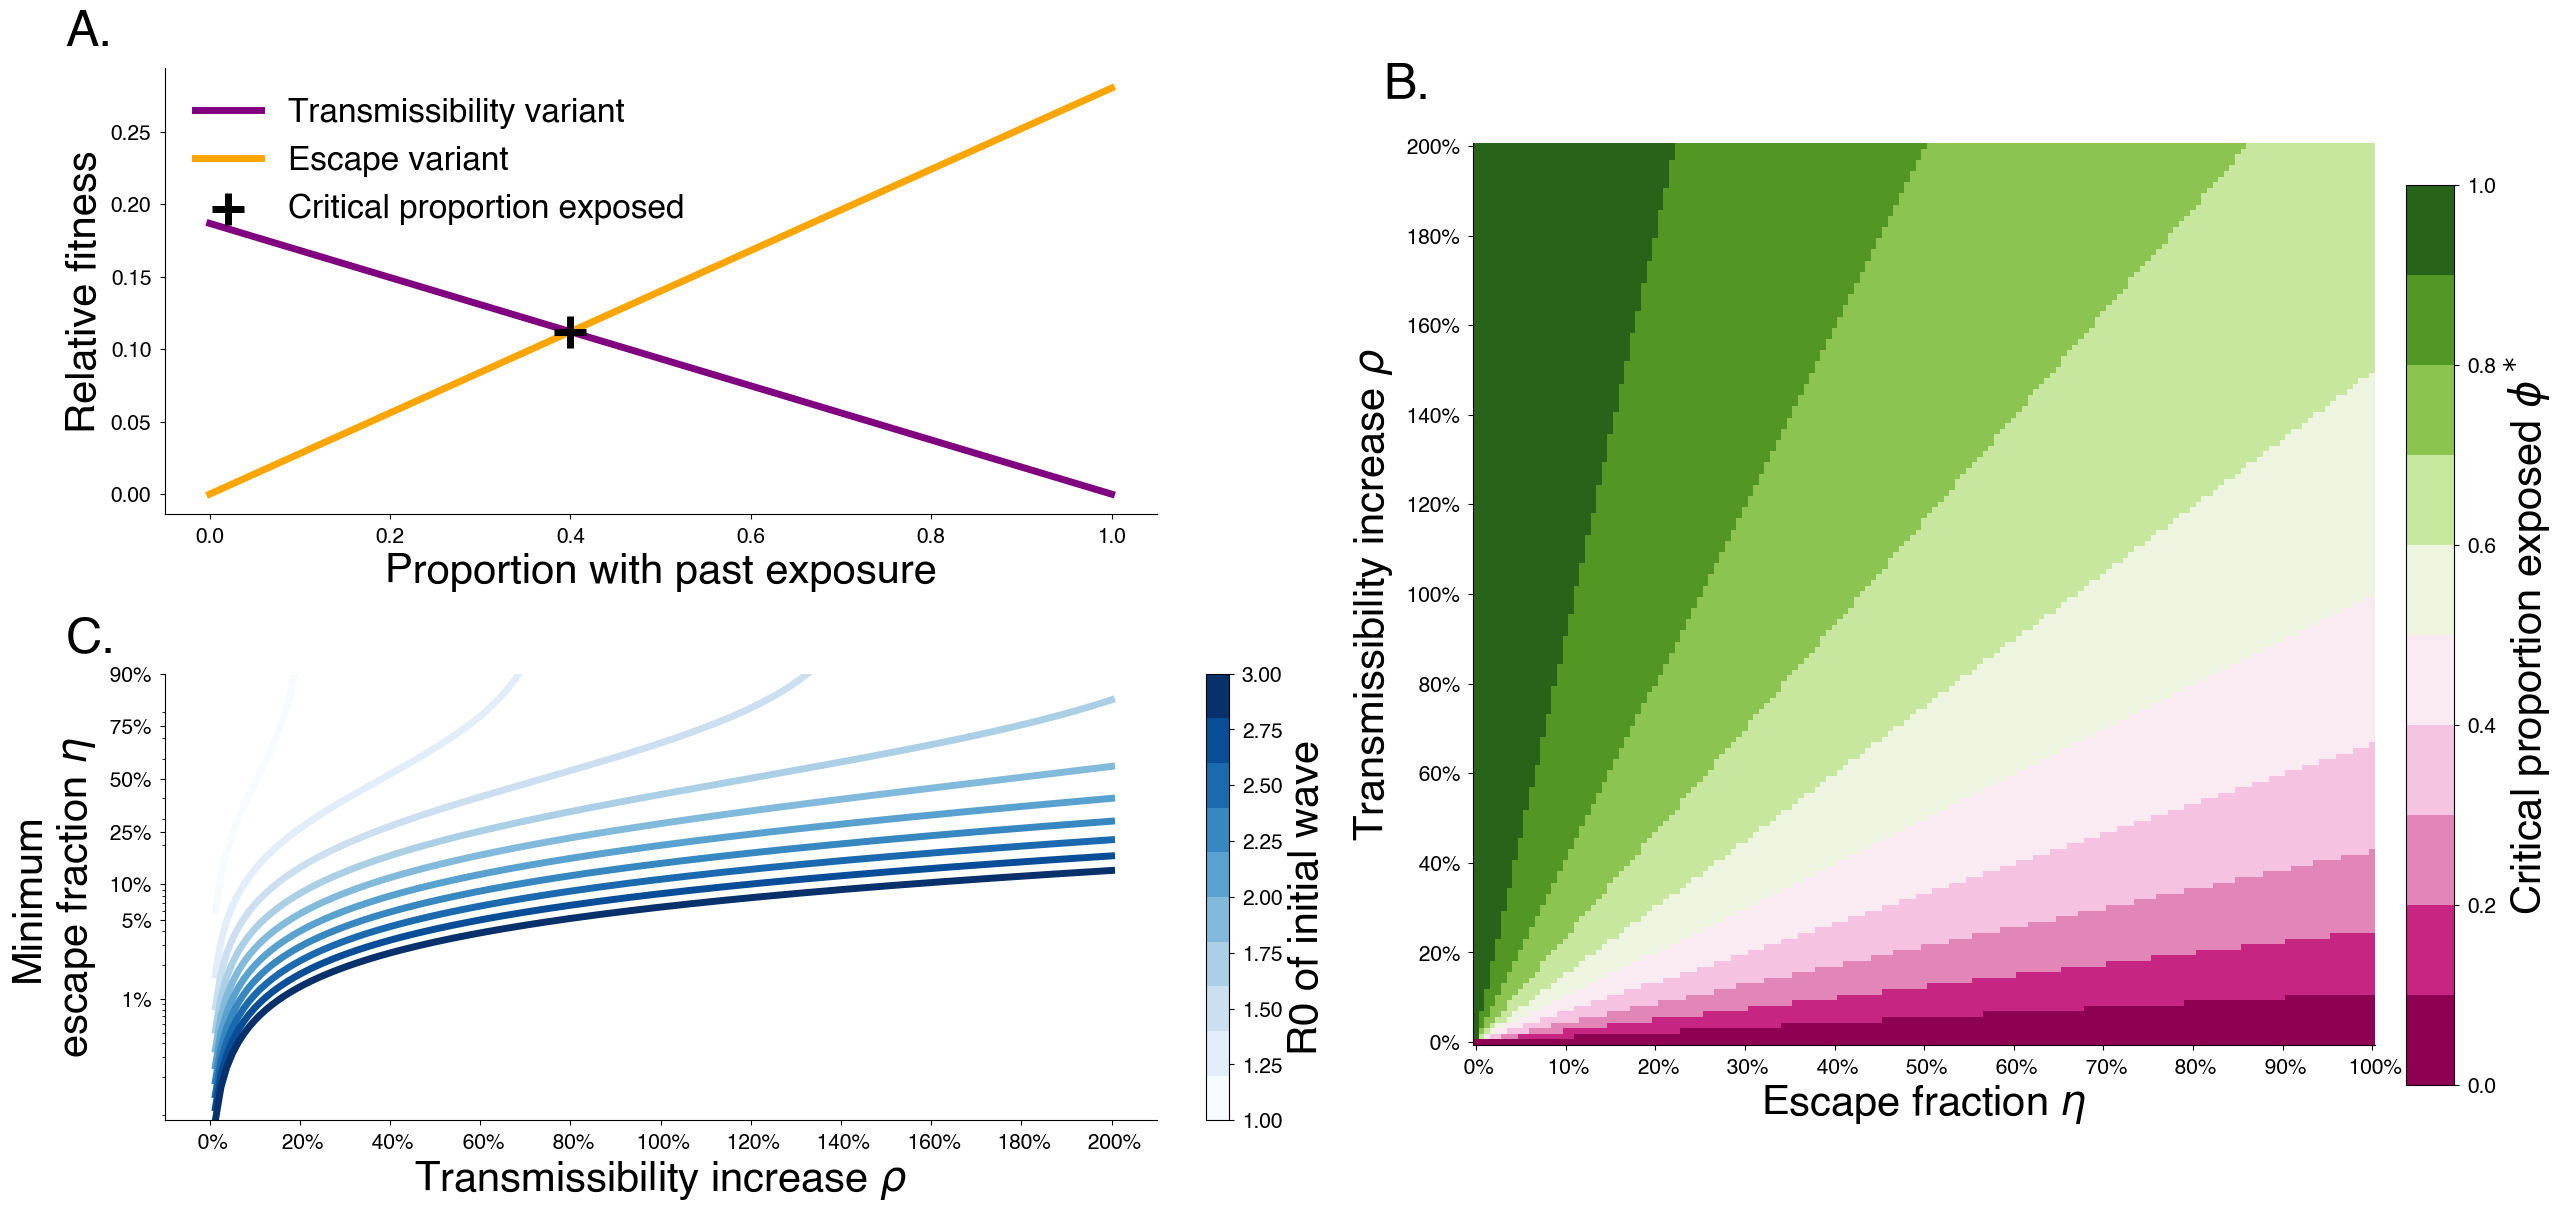
\includegraphics[width=0.8\linewidth]{./figures/transmission_tradeoff.png}
    \caption{\textbf{Trade-off between immune escape and transmissibility increases.}
    A. Relative fitness for a transmissibility increasing variant and an immune escaping variant for $\eta_{T}=0.3$, $\eta_{E}=1.2$, $\beta=0.875$.
    The intersection point shows the point after which the escape variant is has higher fitness.
    B. The critical exposure proportion is shown for various escape fraction and transmissibility increase. Above the critical exposure proportion, we expect dominance of escape variants.
    C. The minimum escape fraction needed for second waves to be comprised of escape variant assuming competition with transmissibility increase variants and first wave with a given $R_{0}$.}
    \label{fig:transmission_tradeoff}
\end{figure}

\paragraph{Initial growth rates are insufficient for predicting short-term frequency growth}%

One question of interest is whether the mechanism meaningful informs our ability to forecast short-term frequency growth.
The first step to addressing this is to understand how the relative fitness may change in time to understand the predictability of relative fitness in the short-term.

To be consistent with the relative fitness framing used through this paper, we model the relative fitness as being the weighted average of several time varying functions $\phi_{b}(t)$ with weights $\beta_{b}$, so that

\begin{align*}
\lambda_{v,u}(t) = \sum_{1 \leq b \leq B} \beta_{b} \phi_{b}(t).
\end{align*}

Even in the case of complete knowledge of the relative fitness and the underlying fitness contributions in the present and past, we have that change in the relative fitness is determined by

\begin{align*}
    \frac{d\lambda_{v,u}}{dt} = \sum_{1 \leq b \leq B} \beta_{b} \frac{d\phi_{b}}{dt}(t).
\end{align*}

By considering a Taylor expansion of the relative fitness about the point of estimation $t_{0}$, we can approximate the relative fitness in the future as:

\begin{align*}
    \lambda_{v,u}(t) \approx \lambda_{v,u}(t_{0}) + \sum_{1\leq b \leq B} (\eta_{v, b} - \eta_{u,b}) \frac{d\phi_b}{dt}(t_0).
\end{align*}

The idea here being that large differences in the form of $\lambda_{v,u}(t)$ can lead to meaningful differences in the future relative fitnesses.
%TODO: However knowledge of the underlying mechanism can inform the evolution of relative fitness

We investigate whether relative fitnesses vary predictably in the short-term regardless of mechanism, so that short-term forecasts are unaffected by mechanistic differences in the assumed transmission process.

To address this, we apply the two-variant model developed in previous sections for two different mechanisms (immune escape and increased transmissibility).
We fix the relative fitness of the novel variant at a prediction time $t_{0}$ using equation \ref{eq:critical_immunity} and assess the change in the relative fitness in the short-term.
We find that though relative fitness trajectories will share the same decreasing shape, they may decline at different rates depending on the mechanism (Fig.~\ref{fig:short_term_divergence}).

This can lead to large changes in the predicted incidence depending on the assumed mechanism and affects to overall rate of turnover.

\begin{figure}[h]
    \centering
    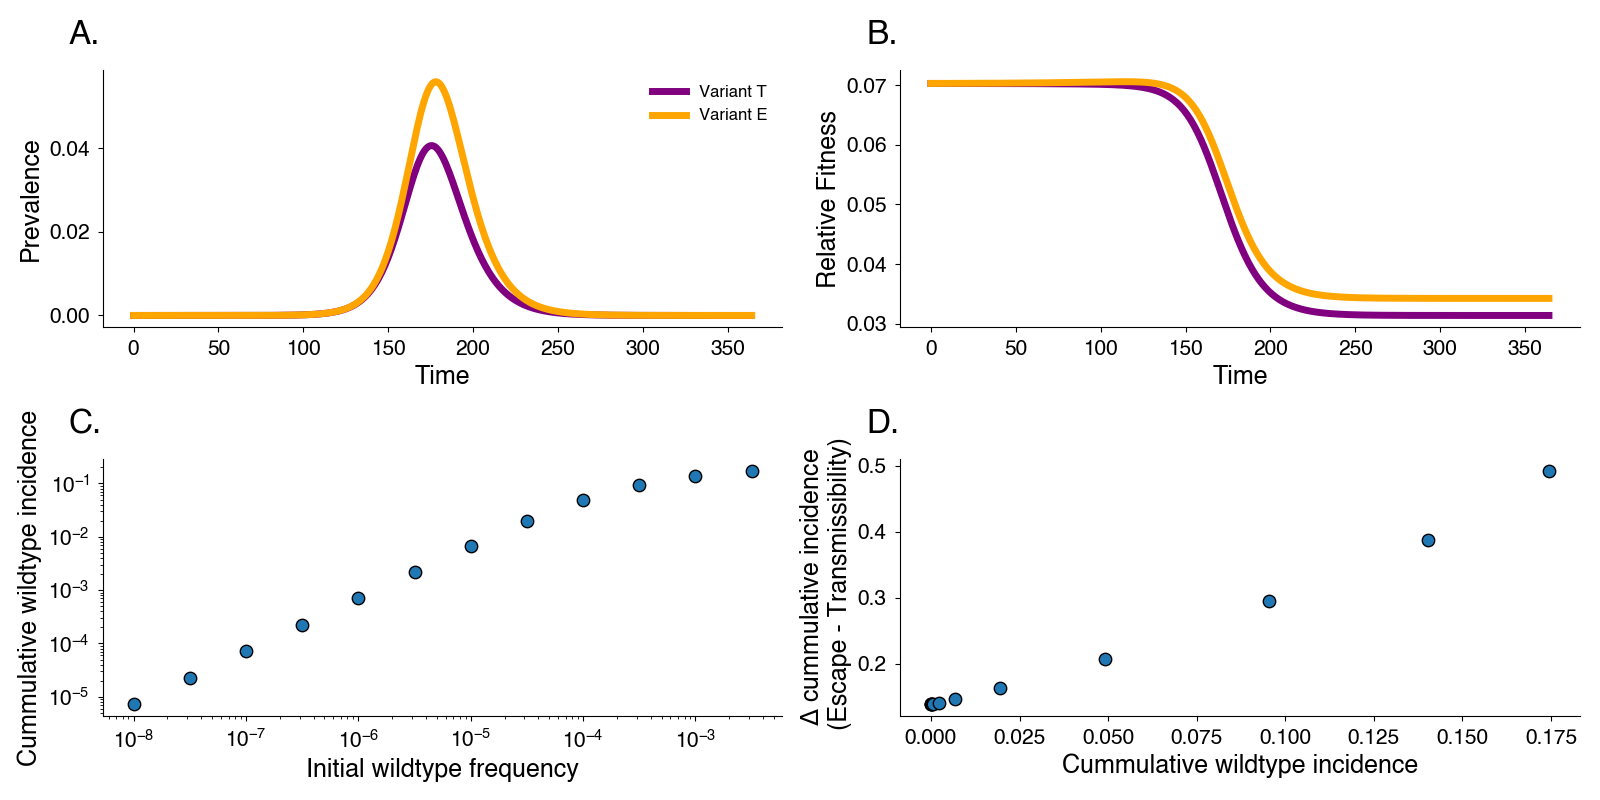
\includegraphics[width=0.8\linewidth]{./figures/short_term_divergence.png}
    \caption{\textbf{Differences in fitness mechanisms impact frequency and prevalence in the short-term.}
    Comparing simulations from two independent two-variant systems with either an escape variant E (orange) or a transmissibility variant T.
    We fix the initial relative fitness for the two variants using Equation \ref{eq:critical_immunity} and simulate dynamics for 365 days.
    (A) The prevalence for the variants.
    (B) The relative fitness from the variants.
    (C) The cumulative wildtype incidence as a function of the initial wildtype frequency.
    (D) The difference between the cumulative incidence between the escape variant and the transmissibility variant as a function of wildtype incidence.
    }%
    \label{fig:short_term_divergence}
\end{figure}

\paragraph{Correlations are insufficient for mechanism identification}%

Variant growth advantages can be correlated with vaccination proportions even in the absence of immune escape.
Simulated multiple epidemics of a pure increased transmissibility variant at varying levels of initial vaccination and was able to see that estimated growth advantages, computed using a logit linear model, were correlated with initial vaccination fraction.

We find that you can estimate association of increased relative fitness due to vaccination in the absence of immune escape.
This appears to hold up until both variants' initial effective reproduction number is below 1 i.e. $V_{0} > 1 / R_{v}$.

\begin{figure}[h]
    \centering
    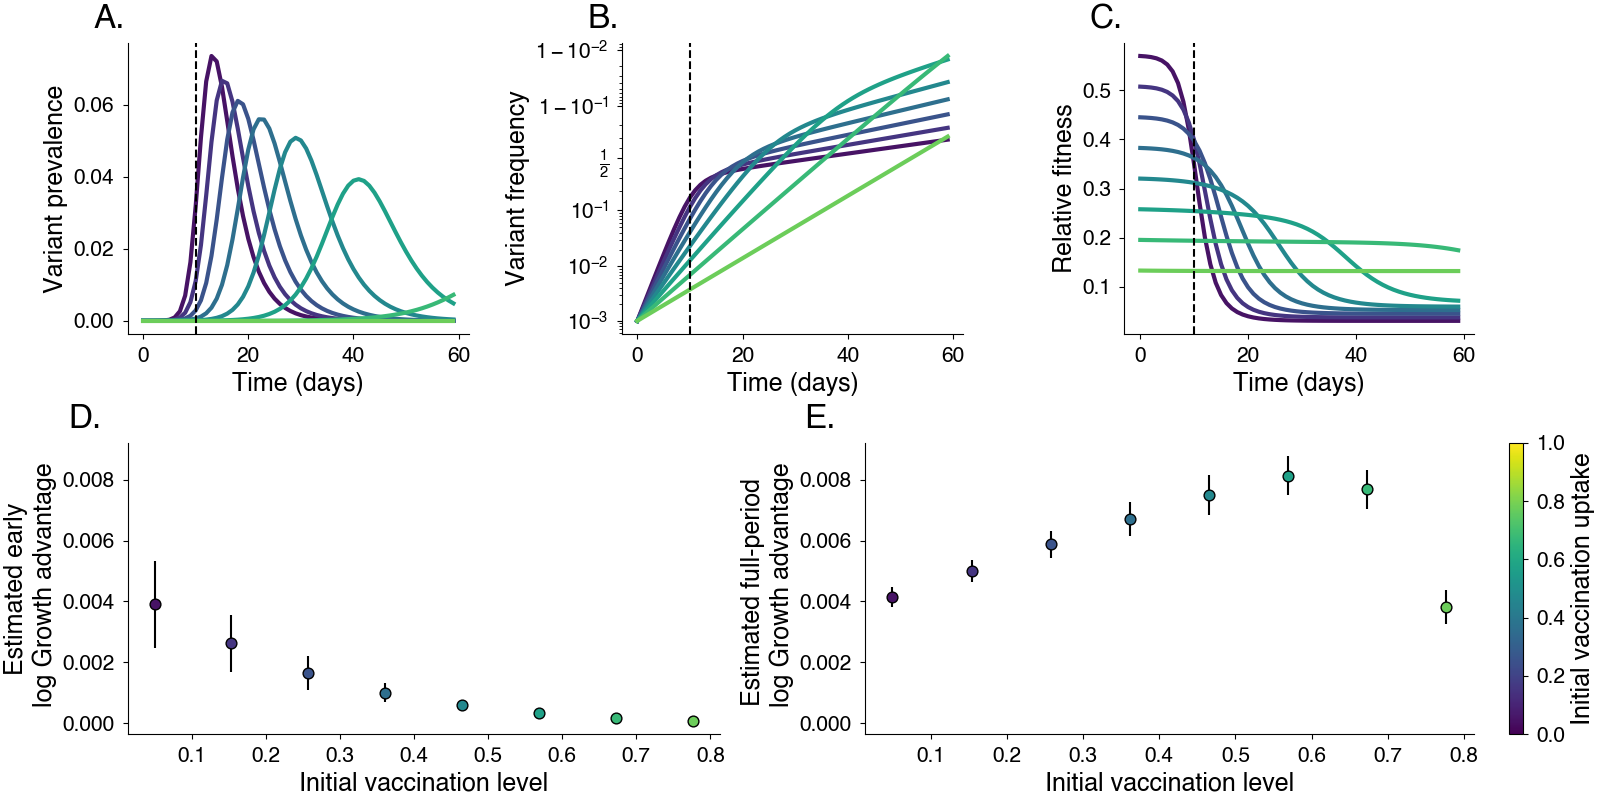
\includegraphics[width=0.8\linewidth]{./figures/correlation_not_mechanism.png}
    \caption{\textbf{Relative fitness is correlated with vaccination levels in the absence of immune escape.}
    We simulate the growth of a pure transmissibility increased variant at varying levels of vaccination.
    Darker colors represent lower vaccine uptake.
    We identify an early growth period where relative fitness is at its highest; the cutoff for this period is denoted with a vertical dashed line.
        A. Prevalence of variant, each line is its own simulation.
        B. Frequency of variant.
        C. Relative fitness for variant over time.
        D. Estimated log growth advantage using linear regression of log relative frequency of variant over wildtype using only data before the early cutoff.
        E. Same as D. but using data from the entire period shown. Notice the drop-off of relative fitness above $1 / R_{v}$ at which both variants are declining.
    }
\label{fig:mechanism_identification}
\end{figure}

\paragraph{Selective Pressure}

Though it is useful to quantify the individual relative fitnesses of individual variants, we are often interested in quantifying the overall effects of selection in the population.
This will occur not just on the level of frequencies and frequency growth, but additionally on the level of population-level growth rates.

Beginning again from our assumption of inhomogeneous exponential growth, we can write a differential equation for the total prevalence $I(t)= \sum_{v} I_{v}(t)$ as

\begin{align*}
    \frac{d I}{d t} &= \sum_{v} \frac{d I_{v}}{d t} =  \sum_{v} r_{v}(t) I_{v}(t)\\
                    &= \left( \sum_{v} r_{v}(t) f_{v}(t) \right) I(t),
\end{align*}

where we've used that $I_{v}(t) = f_{v}(t) I(t)$.
This allows us to see that $\overline{r}(t) = \sum_{v} r_{v}(t) f_{v}(t)$ is the average growth rate of the prevalence.
Re-writing the average in terms of some base exponential growth rate and the relative fitnesses so that $r_{v}(t) = \lambda_{v}(t) + r_0(t)$, we get that $\overline{r}(t) = \sum_{v} \lambda_{v}(t)f_{v}(t) + r_0(t)$.
We can now look at the rate of change in the average growth rate by taking its derivative.

\begin{align*}
    \frac{d \overline{r}}{d t} &= \frac{d r_{0}}{d t} + \sum_{v} \left[\frac{d \lambda_v}{d t} f_{v}(t) + \lambda_{v}(t) \frac{d f_{v}}{d t} \right]\\
                               &= \frac{d r_{0}}{d t} + \sum_{v} \left[\frac{d \lambda_v}{d t} f_{v} + \lambda_{v} f_{v} (\lambda_{v} - \overline{\lambda})  \right]\\
                               &= \frac{d r_{0}}{dt} + \sum_{v} \frac{d \lambda_v}{d t} f_{v}(t) + \sum_{v} \lambda_{v} (\lambda_{v} - \overline{\lambda}) f_{v}\\
                               &= \frac{d r_{0}}{dt} + \sum_{v} \frac{d \lambda_v}{d t} f_{v}(t) + \sum_{v} \lambda_{v}^{2} f_{v} - \overline{\lambda}\sum_{v} \lambda_{v} f_{v}\\
                               &= \frac{d r_{0}}{d t} + \Expect_{f(t)}\left[ \frac{d \lambda_v}{d t}\right] +  \Var_{f(t)}[\lambda_{v}].
\end{align*}

Here, we've written the last line in terms of expectations relative to sampling according to the frequency distribution.
This shows us that the change in the average growth rate of the epidemic can be written in terms of the growth rate of the pivot category, the mean rate of change in the relative fitness, and the variance of the relative fitnesses.
We will call terms which can be computed in terms of quantities derived from frequencies alone the selective pressure and denote it as

\begin{equation}
\psi(t) =  \Expect_{f(t)}\left[ \frac{d \lambda_v}{d t}\right] +  \Var_{f(t)}[\lambda_{v}].
\end{equation}

We can use this idea to directly write the prevalence in terms of the selective pressure and the base growth rate.
First, we define a cumulative selective pressure as
\begin{align*}
\Psi(t) = \int_{0}^{t} \psi(s) ds.
\end{align*}

\begin{align*}
    I(t) &= I(0) \exp\left(\int_{0}^{t} \overline{r}(s) ds\right)\\
         &= I(0) \exp \left(\int_{0}^{t} [r_{0}(s) + \Psi(s)]ds \right).
\end{align*}

\paragraph{Predicting epidemic growth rates using selective pressure}%

Motivated by the relationship between the epidemic growth rate and the selective pressure demonstrated above, we developed a predictive model of the epidemic growth rate using estimates of selective pressure.
Using selective pressure computed using the approximate Gaussian process model, we predict the epidemic growth rate using the selective pressure for the previous 30 days.
We fit a transformer-based model to data from 50 states in the United States between March 2021 and March 2022, reserving data between March 2022 and September 2022 for testing.
Our model is able to replicate patterns seen in estimates of the epidemic growth rates in England derived from ONS data between Jan 2022 and Sep 2022.

%TODO: Estimate correlation between the predictions and the values.

\begin{figure}[h]
    \centering
    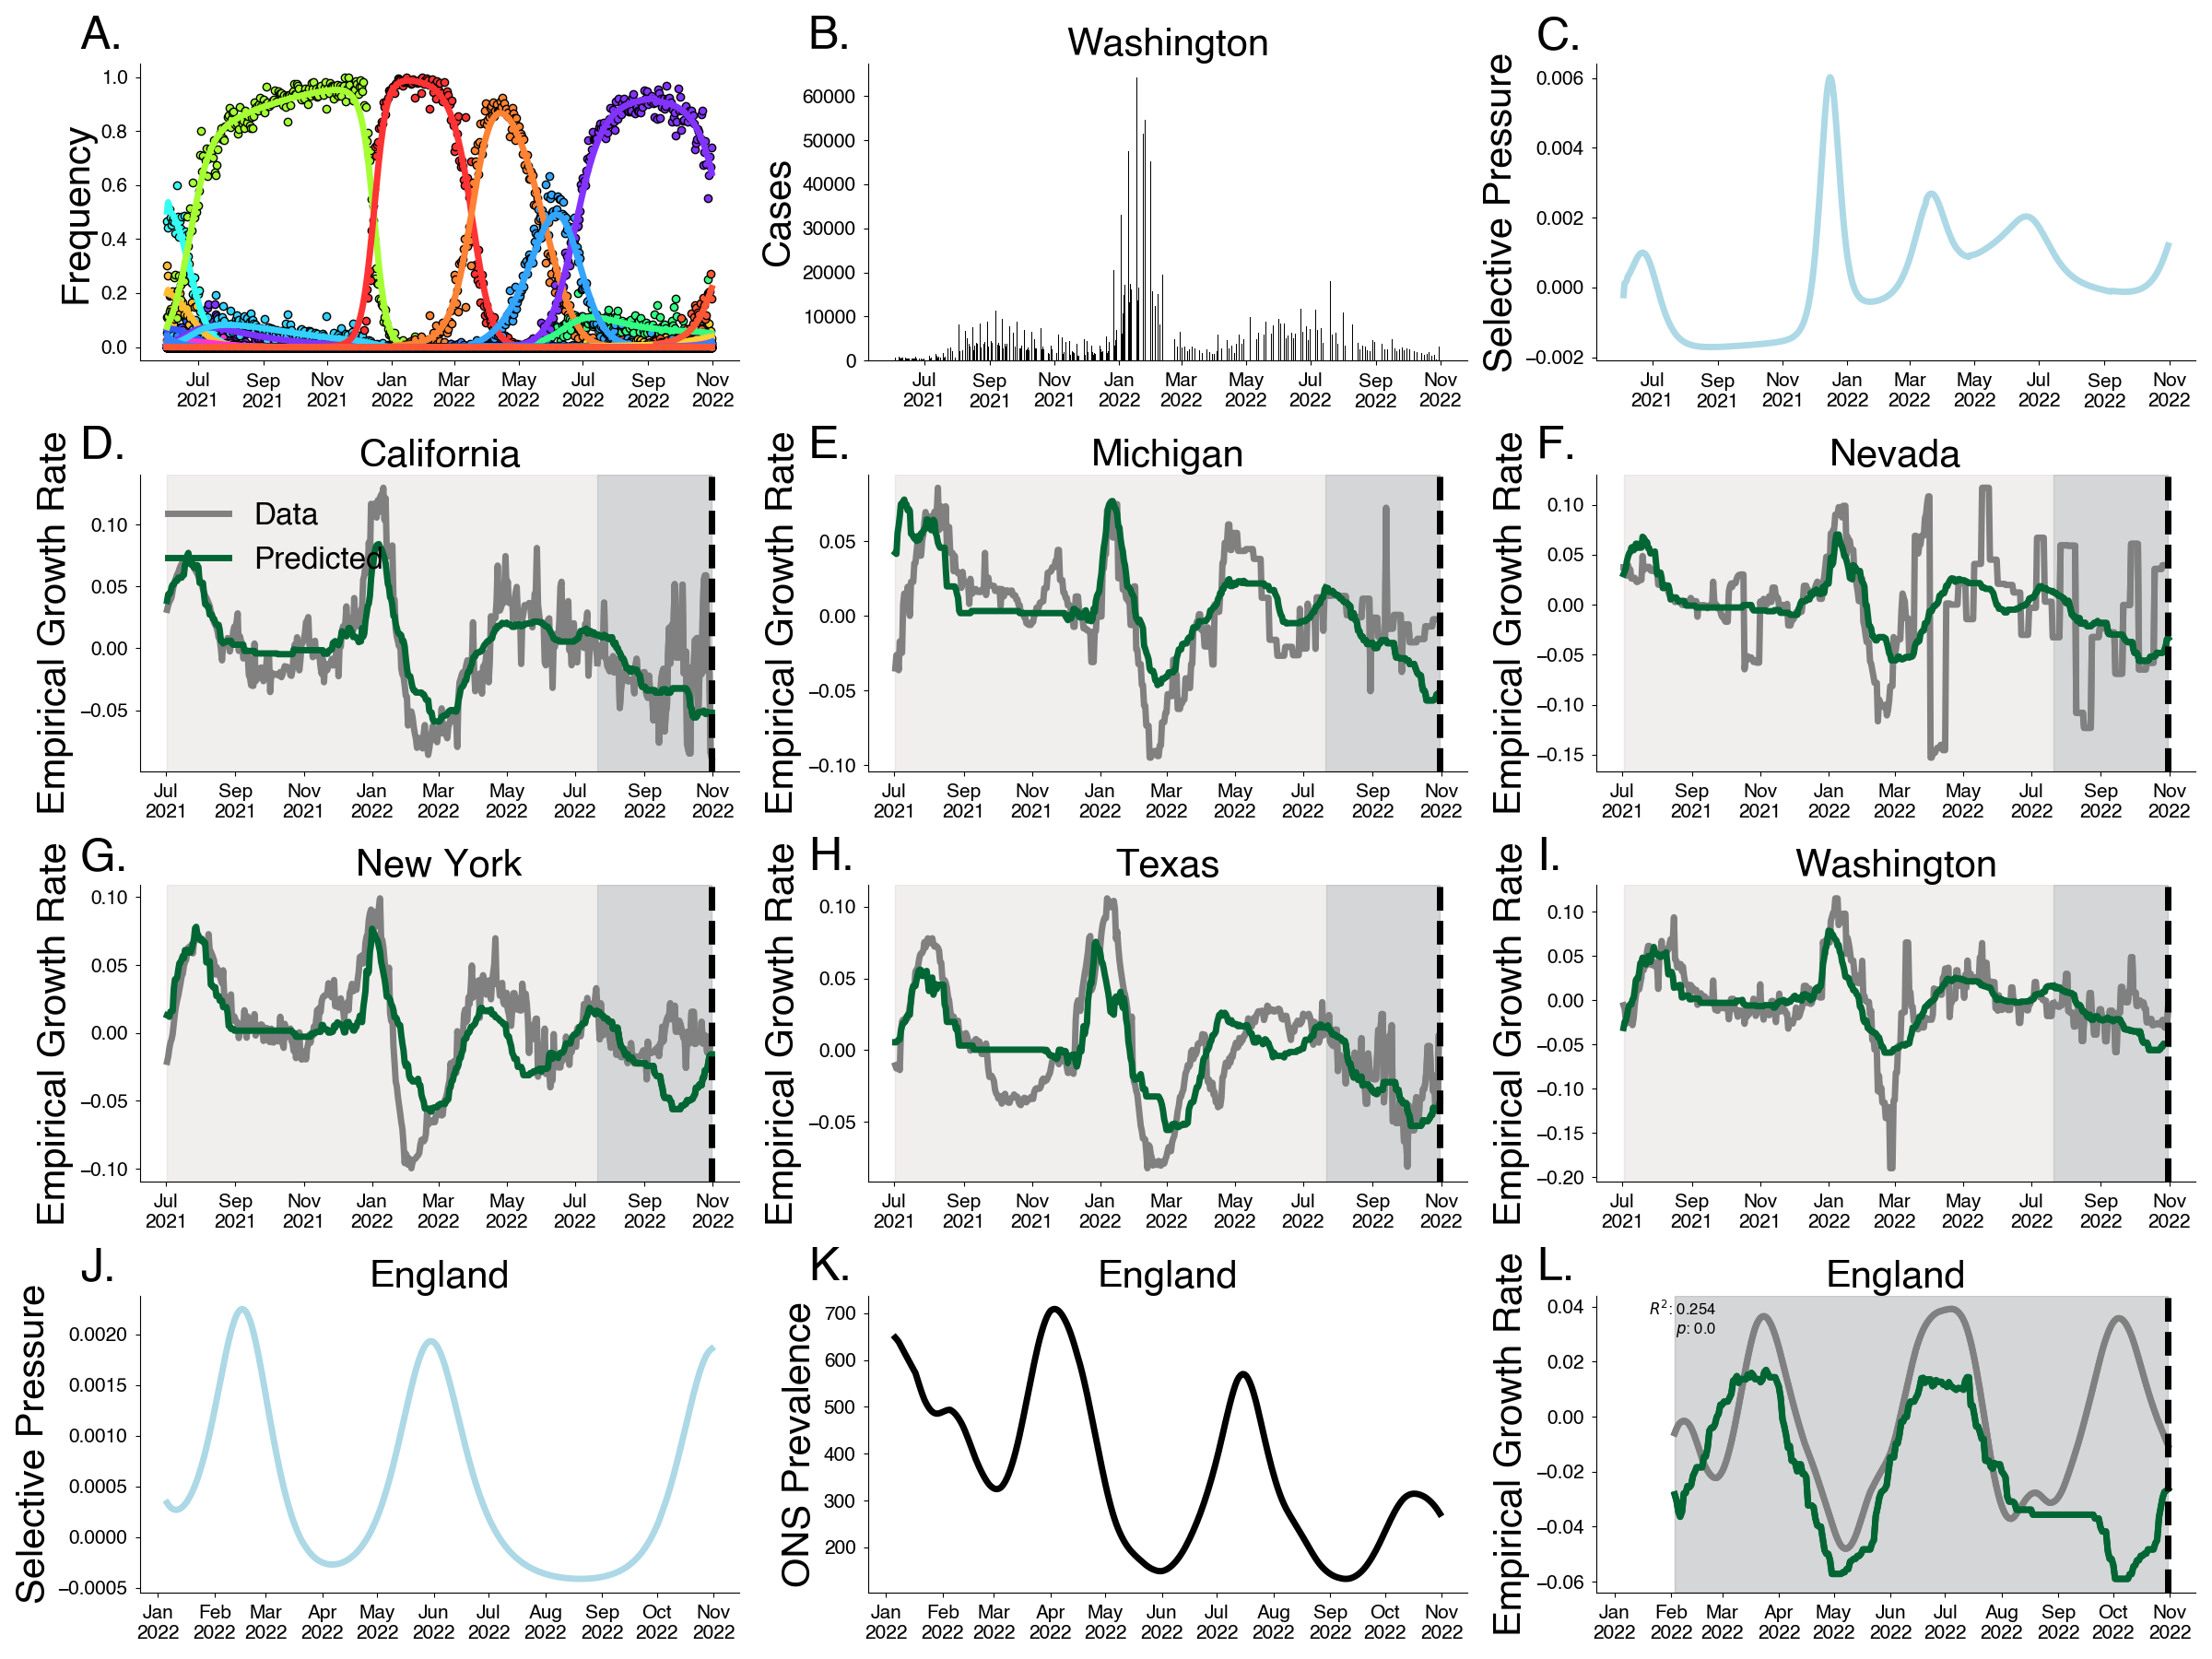
\includegraphics[width=0.8\linewidth]{./figures/selective_pressure_prediction.png}
    \caption{\textbf{Predicting epidemic growth rate using estimated selective pressure.}
    A-F. Predictions for empirical growth rate from selective pressure for selected US states.
    The light gray period is the training period and the darker gray is the testing period.
    G. Estimated selective pressure in England.
    H. Prevalence estimates for England.
    I. Empirical growth rates computed from prevalence estimates in H. and predictions from our model.
}
    \label{fig:selective_pressure_prediction}
\end{figure}

\paragraph{Latent factor models of relative fitness}

The representation of relative fitness using discrete immune backgrounds suggests that there may be low-dimensional structure to variant relative fitness.
To generate pseudo-estimates of this latent factors, we develop and implement our method for latent factors models of relative fitness.

We generate sequence counts for 14 countries and 41 variants in this period, estimating the relative fitness of each variant over time in each country, the pseudo-escape rates for each variant, and the pseudo-immunity for each country.
The results of these models are visualized in Figure \ref{fig:latent_immune} for several selected variants and countries of interest.

We find that the distances in the pseudo-immunity embedding space are correlated with titer differences between variants ($R^2$ = 0.6).

\begin{figure}[h]
    \centering
    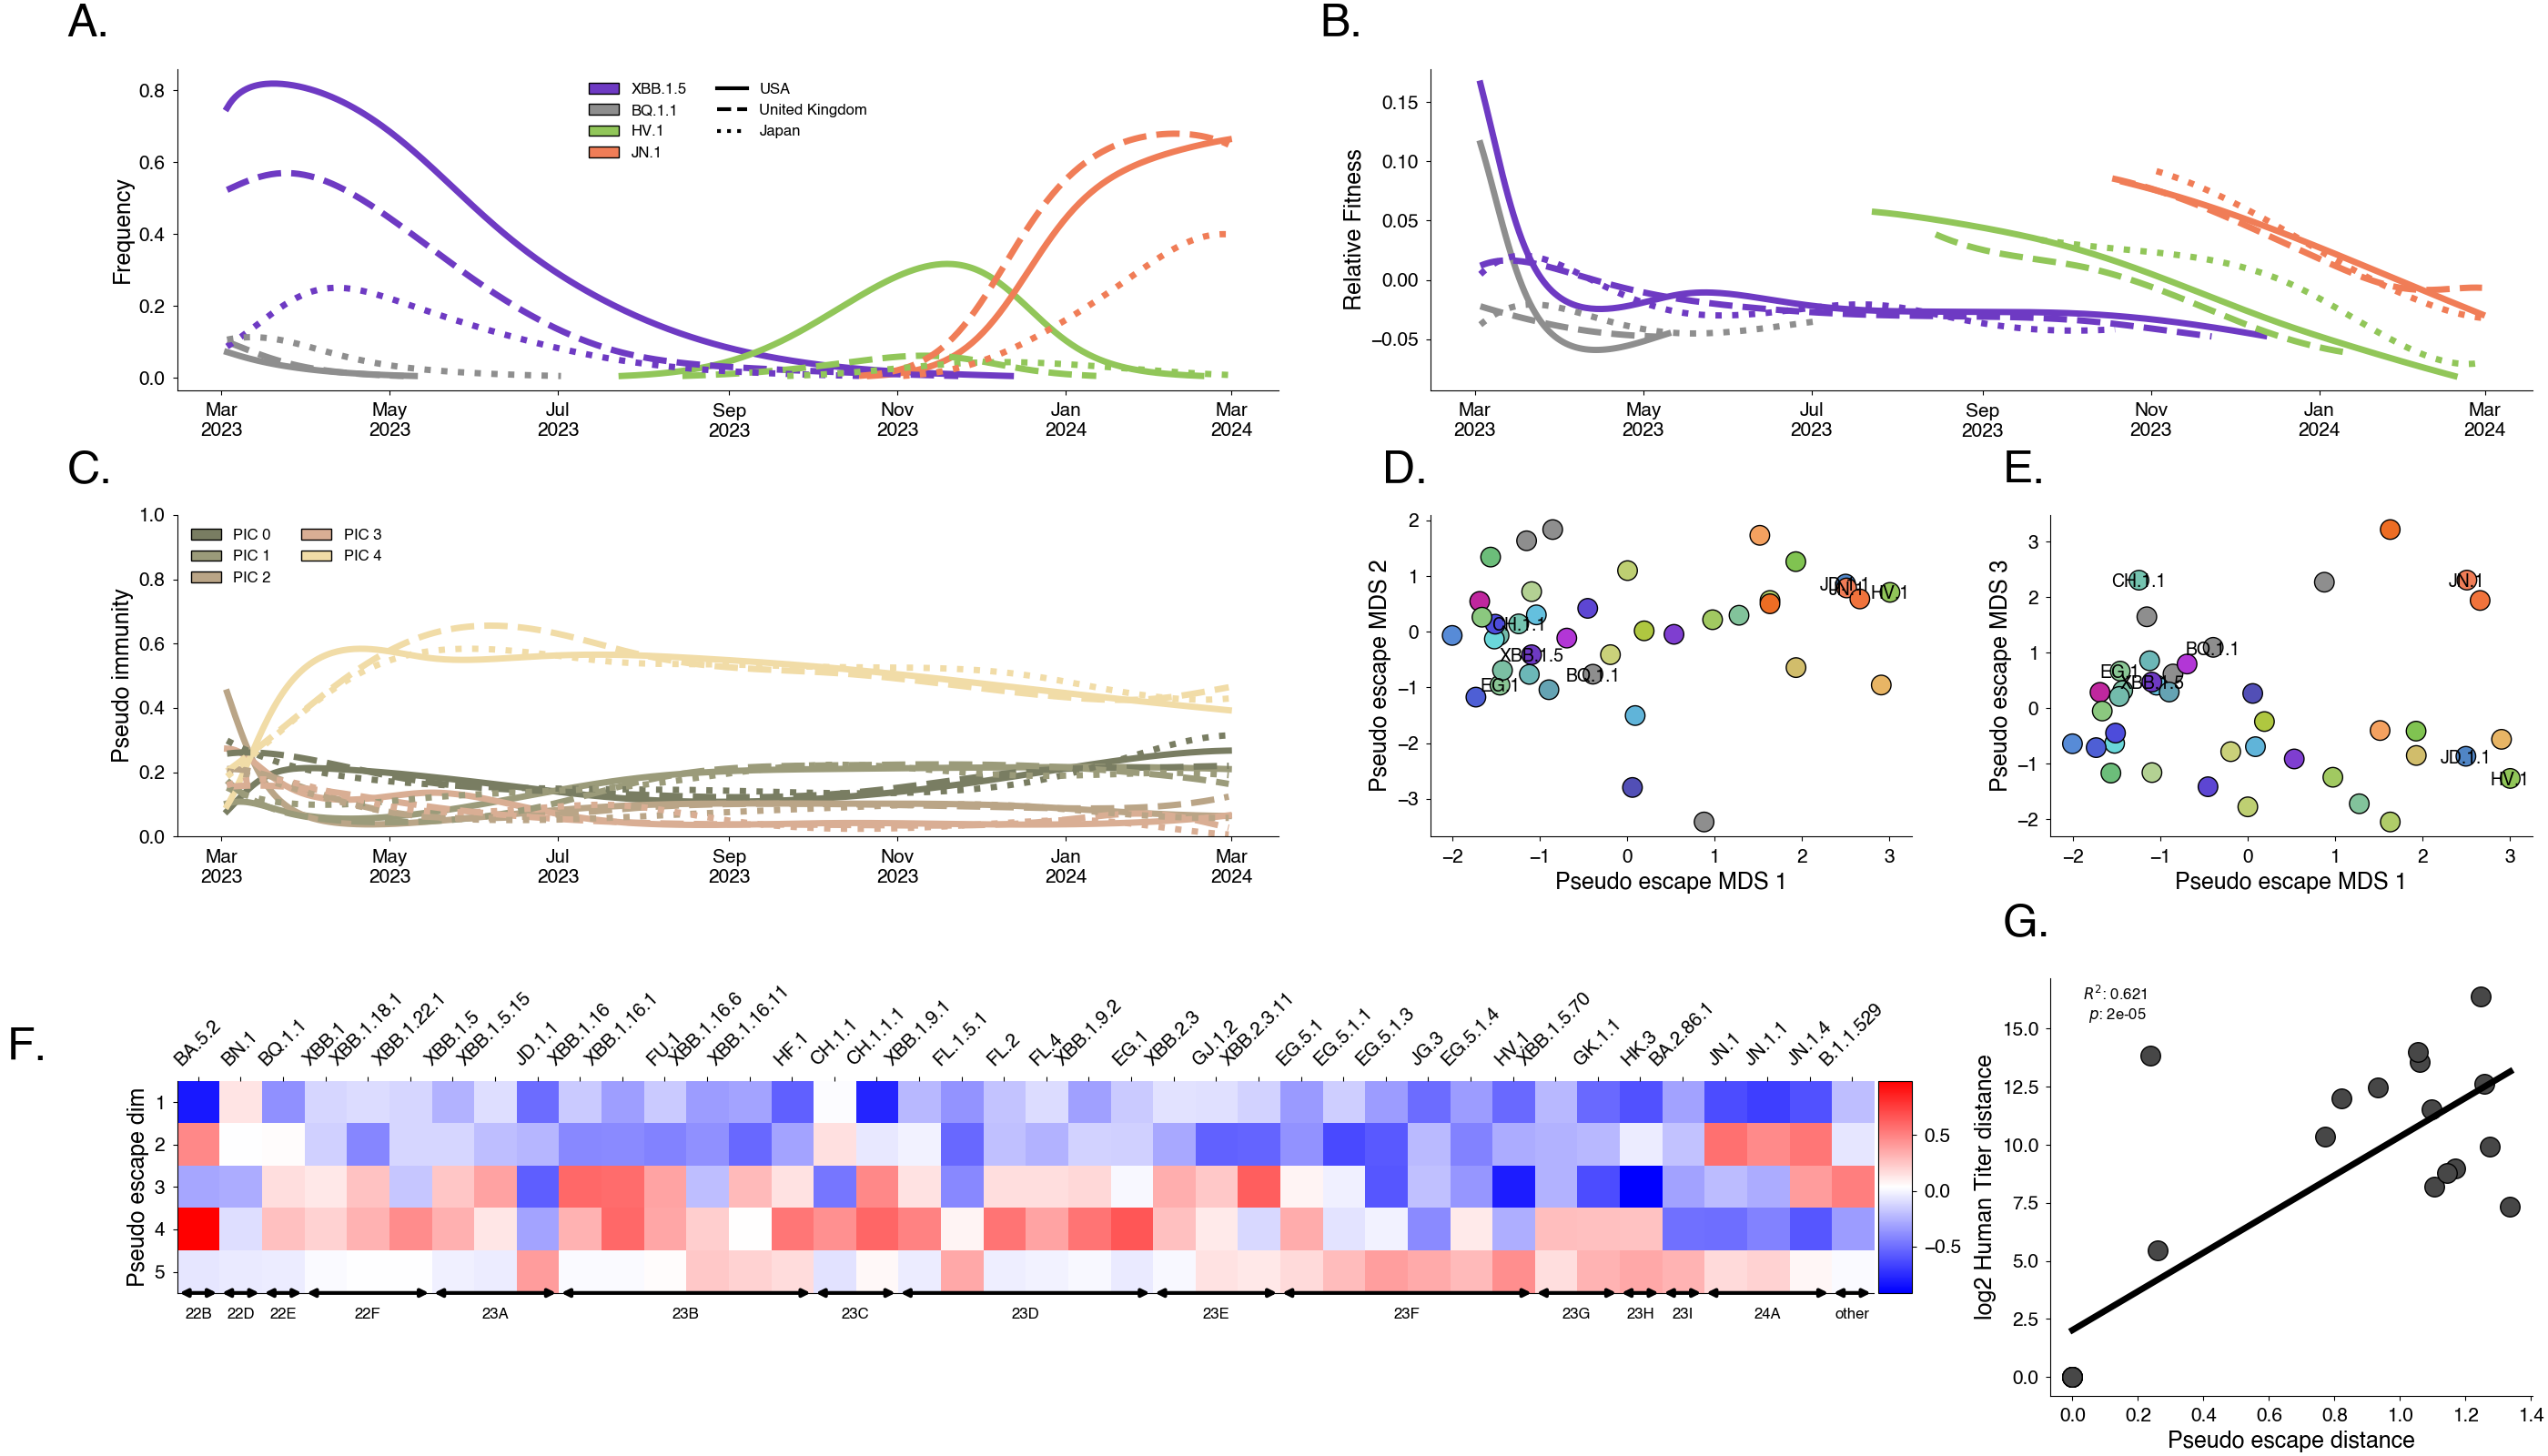
\includegraphics[width=0.8\linewidth]{./figures/latent_immune.png}
    \caption{\textbf{Latent factor models of immunity describe variant structure.}
        We fit the latent immunity factor model to recent SARS-CoV-2 sequence data globally.
        A. Variant frequency. Lines are colored by variant with the style of the line denoting countries of interest.
        B. Estimated relative fitness for selected variants and countries.
        C. Estimated pseudo-immunity over time for multiple countries.
        D, E. Dimensionality-reduced pseudo-escape rates using Multidimensional Scaling.
        F. Estimated pseudo-escape rates for each variant.
        H. Comparing distances in the pseudo-immune space (C) to observed distances in human titer data.
    }
\label{fig:latent_immune}
\end{figure}

\section*{Discussion}

% As is, this is a bit undirected though all valid

% Need to mention models and the way to intrepret results

% Need to mention selective pressure metric, utility of it

% Need to mention benefits of transformer model

% Then neeeed to talk about the limitations, public implementaitons, and donclussion

% Overview of methods

% Mechanistic models
We find that multi-strain mechanistic models of epidemics can be used to inform changes in variant frequency over time.
This enabled us to illustrate the trade-off between intrinsic transmissibility increase and immune escape in environments with heterogeneous past exposure.
These mechanistic models also suggest a structure in which relative fitness is determined by environmental constraints such as the human landscape which we model as several time-varying immunity classes.
Though there appears to be limits to our ability to attribute dynamics to particular mechanisms, the structure of these models suggests that we may improve forecasting by incorporating information about assumed transmission mechanisms or empirically supported mechanisms.
These ideas are already represented in existing literature through the form of long-term forecast models which incorporate phylogenetic and molecular data which is thought to be indicative of selection and immune escape. \cite{Huddleston2020, luksza2014predictive}
Future work should seek to identify and incorporate informative data sources for relative fitness estimation and forecasting for particular pathogens alongside model development.

% Models we developed
In the absence of data that can inform relative fitness, there is still hope.
We find that relative fitness can still be estimated and forecasted in the short-term using frequency data alone.

We develop a scalable approximate Gaussian process model for fitness estimation as well as a latent factor model which decomposes variant advantage into variant pseudo-escape rates and pseudo-immunity proportions.

These models are able to recover pseudo-immunity differences in populations that explain the geographic variation in variant fitness and learn about the structure of immune escape in a way that is consistent with human titer data.
% Though motivated by models of immune escape and well-explined by titer data, latent variable methods may not estimate latent factors that are truly indicative of immune escape directly.

However, it is important to note that these models may not be reliable for longer terms forecasts due to the emergence of new variants or improper specification of mechanism.

% Selective pressure
In the meantime, metrics derived from these models can be informative of much more than just the underlying frequency dynamics.
We define ``selective pressure'' which allows us to model the contribution of evolution to changes in the epidemic growth rate of a population.
This metric allows us to predict the epidemic growth rate using sequence counts alone using machine learning methods and is compatible with all existing methods which estimate frequency and relative fitness.
This provides a simple measure of epidemic growth in the absence of high quality case counts though it can be biased by non-evolutionary effects on the epidemic growth.

%% Latent factor model
% Add parts that highlight the sucess
% These models can still be better extended for short-term forecasts or adapted for longer time horizons.
% For example, to account for more complicated patterns in relative fitness, we can extend the Hilbert Space Gaussian Process models to non-stationary kernels.
%
%


% Limitations of existing simple mechanism models
The compartment models discussed here are described by simple mechanisms and more work is needed to adapt this framework to complicated epidemic models such as those with non-exponential generation times could be useful.
Furthermore, the models considered here are primarily deterministic in nature and do not explicitly model the emergence of variant viruses only the dynamics after their successful introduction.

In reality, there are biological constraints on the types of variants that are produced in nature and even if there is a "true" fitness boost, the chance for stochastic extinction of beneficial variants remains.
That being said, models which account for the appearance of genetic variants through mutation exist, often assuming a latent antigenic space with which fitness is determined.

Despite the limitations discussed above, the framework presented here illustrates the importance of transmission mechanism in the evolution of pathogens, highlighting the importance of both variant characteristics and population susceptibility in selection.
We suggest that future models of pathogen transmission and evolution attempt to incorporate current knowledge of the transmission process into their forecasts.

In particular, for viruses such as influenza and SARS-CoV-2 which undergo antigenic evolution, our work suggests that incorporating knowledge on both the diversity in human immune response and the escape potential of emerging variants could prove useful in improving long-term forecasts of the viral population.

%TODO: Borader implications, detailed landscapes, robust framework

\section*{Methods}

\paragraph{Generating sequence counts}%

We prepared sequence count data sets using the Nextstrain-curated SARS-CoV-2 sequence metadata \cite{Hadfield2018} which is created using the GISAID EpiCoV database \cite{khare2021gisaid}.
These sequences were tallied according to either their annotated Nextstrain clade or Pango lineage depending on the data set to produce sequence count for each variant, for each day over the period of interest, and in each location analysed.

\cite{aksamentov2021nextclade}

\paragraph{Likelihood of sequence counts given frequencies}

The models discussed in this paper use counts of variant sequences to inform the underlying variant frequency in the population.
This is accomplished using a multinomial likelihood, so that given counts of sequences $C_{t,v}$ of variant $v$ at time $t$ and total sequences $N_{t}$ collected at time $t$, we have that

\begin{equation*}
    C_{t, \cdot} \sim \text{Multinomial}(N_{t}, f_{v}(t)),
\end{equation*}

where $f_{v}(t)$ is the frequency of variant $v$ at time $t$.
This is a simple model of sequence counts to frequencies and does not account for over-dispersion of sequence counts relative to a multinomial, however, all models can be extended to estimate and account for over-dispersion by replacing the above likelihood with a Dirichlet-Multinomial likelihood.

\paragraph{Approximate Gaussian processes for relative fitness estimation}%

To generate smooth non-parametric estimates of variant growth rates, we develop a Gaussian process based model for relative fitnesses.
That is, we model the relative fitness for each variant $v$ over time as a multivariate normal distribution:

\begin{align*}
    \vec{\lambda}_{v} &\sim \text{Normal}(\vec{\mu}, \vec{\Sigma})\\
    \vec{\Sigma}_{s, t} &= K_{\theta}(s, t),
\end{align*}
where $K_{\theta}$ is a potentially parameterized kernel function.
This induces a structure on the covariance of the relative fitness values over time.

For computational efficiency, we implement a Hilbert Space Gaussian process approximation, so that the relative fitnesses can be represented linearly as

\begin{equation}
    \lambda_{v}(t) \approx \sum_{j=1}^{m} S_{\theta}(\sqrt{\mu_{j}})^{1/2} \cdot \phi_{j}(t) \cdot \beta_{j},
\end{equation}
where $S_{\theta}$ is the spectral density of the kernel $K_\theta$, $\mu_{j}$ and $\phi_{j}$ are the eigenvalues and eigenfunctions of the Laplacian, and $\beta_{j} \sim \text{Normal}(0,1)$ \cite{riutortmayol2022practical}.
Since the eigenvalues and eigenfunctions are shared across variants, this allows us to re-use values across variants, simplifying the computation to a matrix multiplication as

\begin{equation*}
    \vec{\lambda}_{t} = \vec{\Phi}_{t} \sqrt{\vec{S}_{\theta}}\vec{\beta}.
\end{equation*}

\paragraph{Predicting epidemic growth rate from selective pressure}%

The derivation of the selective pressure metric shows that the selective pressure can be a useful tool in predicting the epidemic growth rate.
To develop a predictive model of epidemic growth rate using selective pressure, we begin by generating estimates of selective pressure and epidemic growth rate from a period with high sequencing and case surveillance.

We take sequence count and case count data from the United States between March 2021 and March 2022.
Using the sequence counts, we compute selective pressure estimates from relative fitness and frequencies estimated with our approximate Gaussian process relative fitness model.

From the case data, we derive the empirical growth rate using a 7-day moving average on case counts $\hat{C}_{t}$ and computing the empirical growth rate as $\hat{r}_{t} = \log(\hat{C}_{t}) - \log(\hat{C}_{t})$.

We then use the past 14 days of selective pressure to predict the empirical growth rate using a transformer-based model.
Our model uses a loss function which weights the mean absolute error and a smoothness loss on predicted trajectories.
\begin{equation*}
    \text{loss} = \text{MAE}(\hat{y}, y) + \alpha \text{Smoothness}(\hat{y}),
\end{equation*}
where $\alpha = 1\times 10^{-6}$ and $\text{Smoothness}(y) = \frac{1}{T}\sum_{t=1}^{T} (y_{t+1} - 2 y_{t} + y_{t+1})^{2}$.
We fit this model using an AdamW optimizer with learning rate LEARNING RATE for NUM EPOCHS epochs.

We validate our model by comparing our predicted epidemic growth rates to estimates of the epidemic growth rates in England derived from ONS data between Jan 2022 and Sep 2022.
As a baseline, we compare the results of this model to linear regression, lasso, ridge regression, and gradient boosted trees.

% Mention data source for training and evaluation data

% Mention model specification, cross-validation, and ...

\paragraph{Latent immune factor model}%

We show that relative fitness dynamics ought to be explained by low-dimensional immunity when transmission dynamics are described with compartment models.
This motivated a model to learn this low-dimensional structure that is inspired by latent-factor models.
We start by assuming that the relative fitness of variant $v$ at time $t$ and in geographic location $g$ can be described by $D$ latent factors so that

\begin{equation}
    \lambda_{v}^{g}(t) = \sum_{d=1}^{D} \eta_{v,d} \phi_{d}^{g}(t).
\end{equation}
As the structure here resembles Equation~\ref{eq:escape_relative_fitness}, we call the $\eta$ ``pseudo-escape'' and $\phi_{d}^{g}$ the ``pseudo-immunity''.
To make this more consistent with our intuition here, we model $\phi_{d}^{g}$ to be in $[0,1]$ and model it as smoothly varying in time.
In the results shown above, we model $\text{logit}(\phi_{d}^{g})$ using 4th order splines with 6 knots placed uniformly over the time period modeled.
Though we choose to model these latent factors with splines, other models would work here. 
For example, one alternative would be the approximate Gaussian processes described above.
Additionally, in order to ensure identifiability of the parameter estimates, we fix some base variant $v^*$ which fitness is defined relative to, so that $\eta_{v^*, d} = 0$ for all $1\leq d\leq D$.
For the same reason, we order the components in the first geography.

We apply this model to SARS-CoV-2 sequence counts in the period between March 2023 to March 2024.

We compare the distances between variant pairs in our estimated pseudo-escape space to distances in log2 titer.

\subsection*{Data and code accessibility}

Source code used to generate figures, model implementations, and sequence count data are available at https://github.com/blab/relative-fitness-mechanisms.

\subsection*{Competing interests}%

\subsection*{Author contributions}
MF conceived the study.
MF, TB gathered sequence and case count data.
MF designed and implemented the models.
MF performed the analysis.
MF, TB interpreted the results.
MF, TB wrote the paper.


\subsection*{Acknowledgements}%

\bibliographystyle{plos}
\bibliography{relative-fitness-mechanisms}

\newpage

\appendix

\setcounter{figure}{0}
\setcounter{table}{0}
\setcounter{page}{1}
\renewcommand{\thefigure}{S\arabic{figure}}
\renewcommand{\thetable}{S\arabic{table}}
\renewcommand{\thepage}{S\arabic{page}}
\renewcommand{\thesubsection}{S\arabic{subsection}}

\section*{Supplemental Appendix}

\subsection{Relative fitness for full immune history models}\label{ssec:full_immune_history}

%TODO: Define powers sets + macro to simplify?
% $\mathcal{P}(M \setminus \{i\})$

We show that the simple background model is consistent with an expanded immune history model.
Beginning with the model from Lazebnik and Bunimovich-Mendrazitsky 2022 \cite{Lazebnik2022}, we consider the differential equation for the individuals with strain infection history $J$ and current infecting strain $i$ $R_{J}I_{i}$
\begin{align*}
\frac{dR_{J} I_{i}}{dt} = - \gamma_{J, i} R_{J} I_{i} + \beta_{J, i} R_{J} \sum_{K \in P(M), i\notin K} R_{K}I_{i}.
\end{align*}

Here, infection can occur from any individual infected with strain $i$ assuming their past immune history does not include $i$ and the infected are any recovered individual with immune history $J$  $R_{J}$.
To compute the strain growth rate, we can sum over all possible immune histories for individuals infected with strain $i$, so that
\begin{align*}
    \frac{d I_{i}}{d t} &= \sum_{J \in P(M), i \notin J} \frac{dR_{J} I_{i}}{dt} \\
                        &= - \gamma_{i} I_{i} + \sum_{J \in P(M), i \notin J} \beta_{i, J} R_{J} \sum_{K \in P(M), i\notin K} R_{K}I_{i}\\
                        &= - \gamma_{i} I_{i} + \sum_{J \in P(M), i \notin J} \beta_{i, J} R_{J} I_{i}\\
                        &= \left(-\gamma_{i} + \sum_{J \in P(M), i \notin J} \beta_{i,J} R_{J} \right) I_{i}\\
                        &= \left(-\gamma + \beta\sum_{J \in P(M), i \notin J} \eta_{i,J} R_{J} \right) I_{i}\\
\end{align*}

Assuming that the transmission rate can be decomposed as a base transmission rate $\beta$ and a strain $i$ and immune history $J$ specific escape rate $\eta_{i, J}$ and that the recovery rate is constant, we notice this is identical to our previous immune background model.
Therefore, our relative fitnesses can be written as

\begin{align*}
    \lambda_{i, j} = \beta \sum_{B \in P(M)} (\eta_{i, B} - \eta_{j, B}) R_{B},
\end{align*}
where for simplicity we define $\eta_{v, B} = 0$ if $v \in B$.

    \begin{figure}[t!]
        \centering
        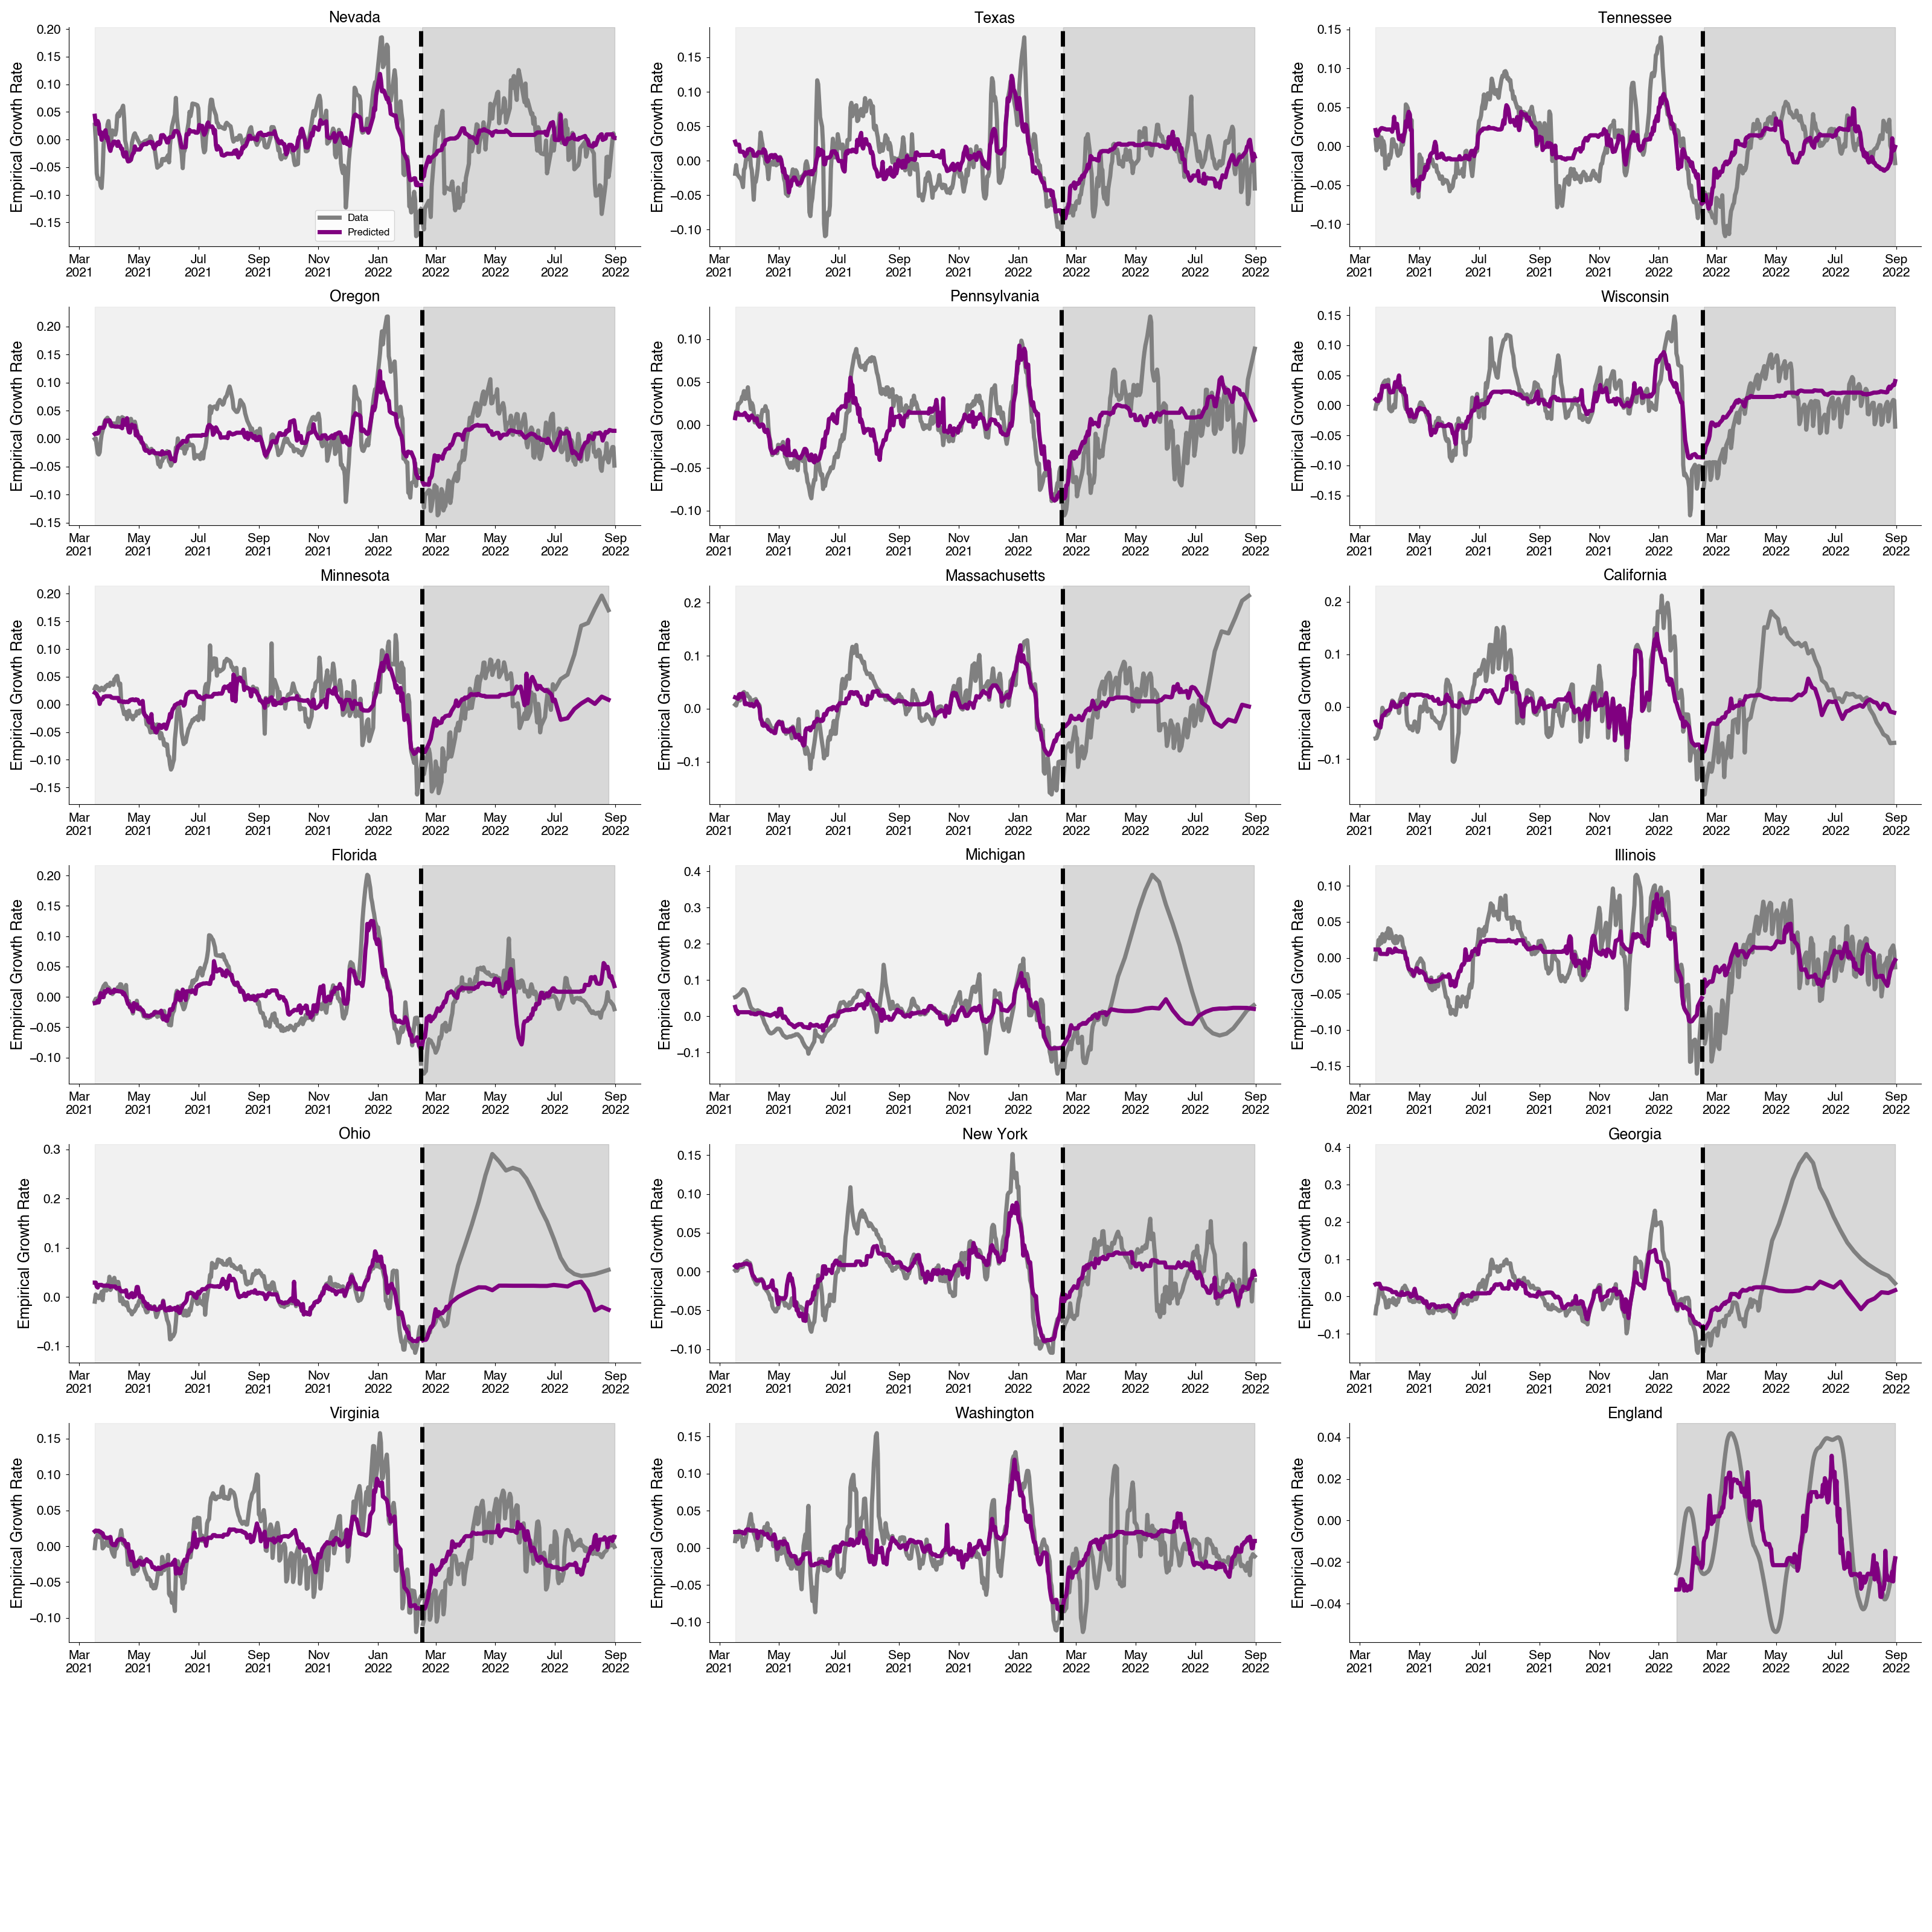
\includegraphics[width=0.9\textwidth=0.01]{./supplementary_figures/empirical-growth-rate-predictions-all.png}
        \caption{
            \textbf{Predictions for empirical growth rate using selective pressure for all locations.}
        }
        \label{fig:empirical-growth-rate-predictions-all}
    \end{figure}
\end{document}
